\documentclass[aspectratio=169,9pt]{beamer}

\usepackage{graphicx,caption,subcaption,hyperref,amsmath,tikz}
\graphicspath{ {./figures/} }
\captionsetup{font=scriptsize,labelfont=scriptsize}
\setbeamerfont{footnote}{size=\scriptsize}
\usepackage[strict]{changepage}
\usetikzlibrary{arrows,automata,positioning}
\usetheme[titleformat=smallcaps,
            sectionpage=progressbar,
			subsectionpage=progressbar,
			progressbar=frametitle,
			numbering=fraction]{metropolis}
% \usecolortheme{owl}
\usepackage[style=apa,
			sorting=nyt,
			date=year,
			bibencoding=utf8,
			isbn=false,
			eprint=false,
			dashed=false,
			uniquelist=false,
			maxbibnames=10,
			minbibnames=1,
			maxcitenames=2,
			uniquename=init,
			giveninits=true,
			useprefix=false,
			minsortnames=1,
			maxsortnames=2]{biblatex}
\bibliography{References}

% Information to be included in the title page:
\title{Deciphering the landscape of cell states in Glioblastoma}
\author{Harshavardhan BV}
\date{\today}
\institute{IISc Bangalore}

\begin{document}
    \frame{\titlepage}

    \begin{frame}{ssGSEA/AUCell}
        \begin{adjustwidth}{-5cm}{-5cm}
            \centering
            \begin{figure}
                \centering
                \begin{subfigure}[b]{0.38\textwidth}
                    \centering
                    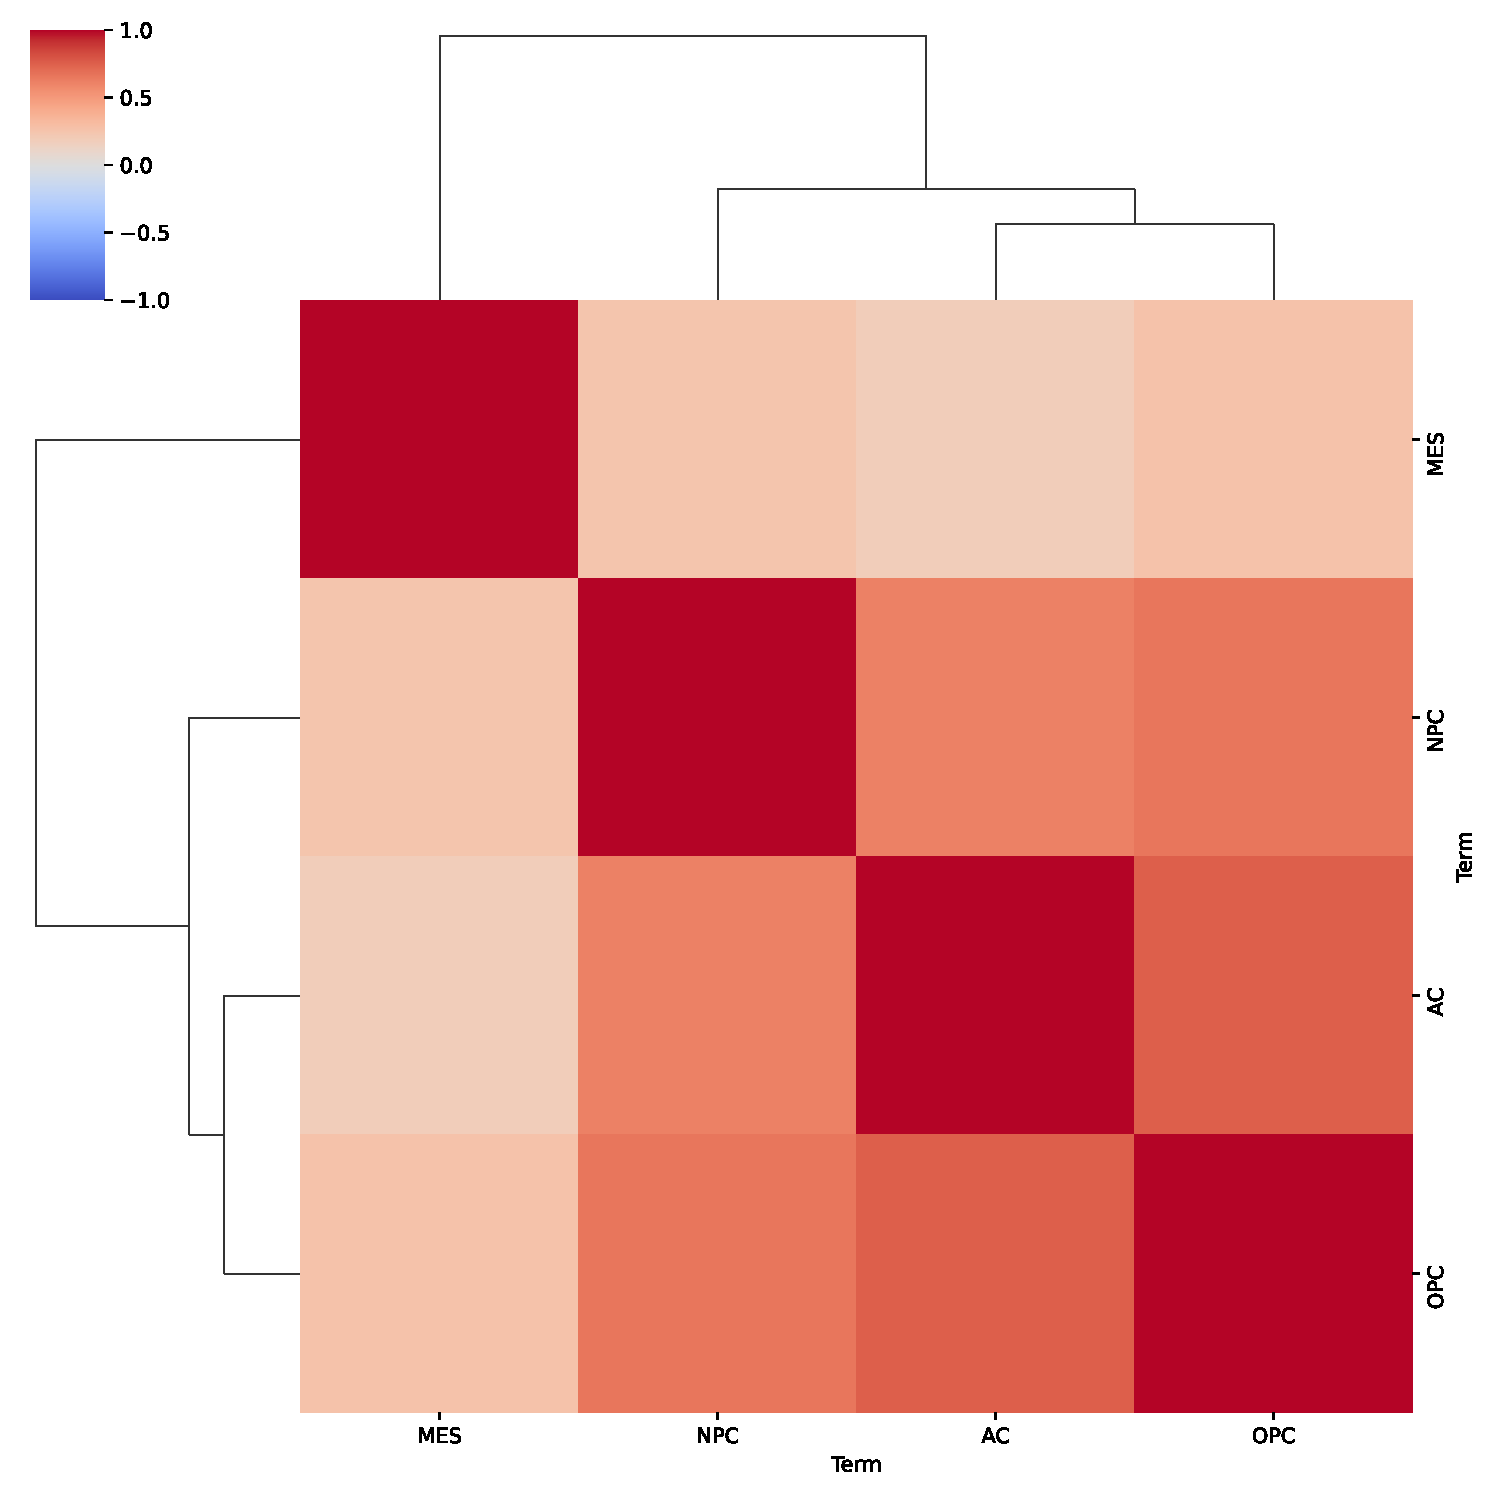
\includegraphics[width=\textwidth]{CCLE_ssgsea_corr_4D}
                    \caption{CCLE}
                \end{subfigure}
                \begin{subfigure}[b]{0.38\textwidth}
                    \centering
                    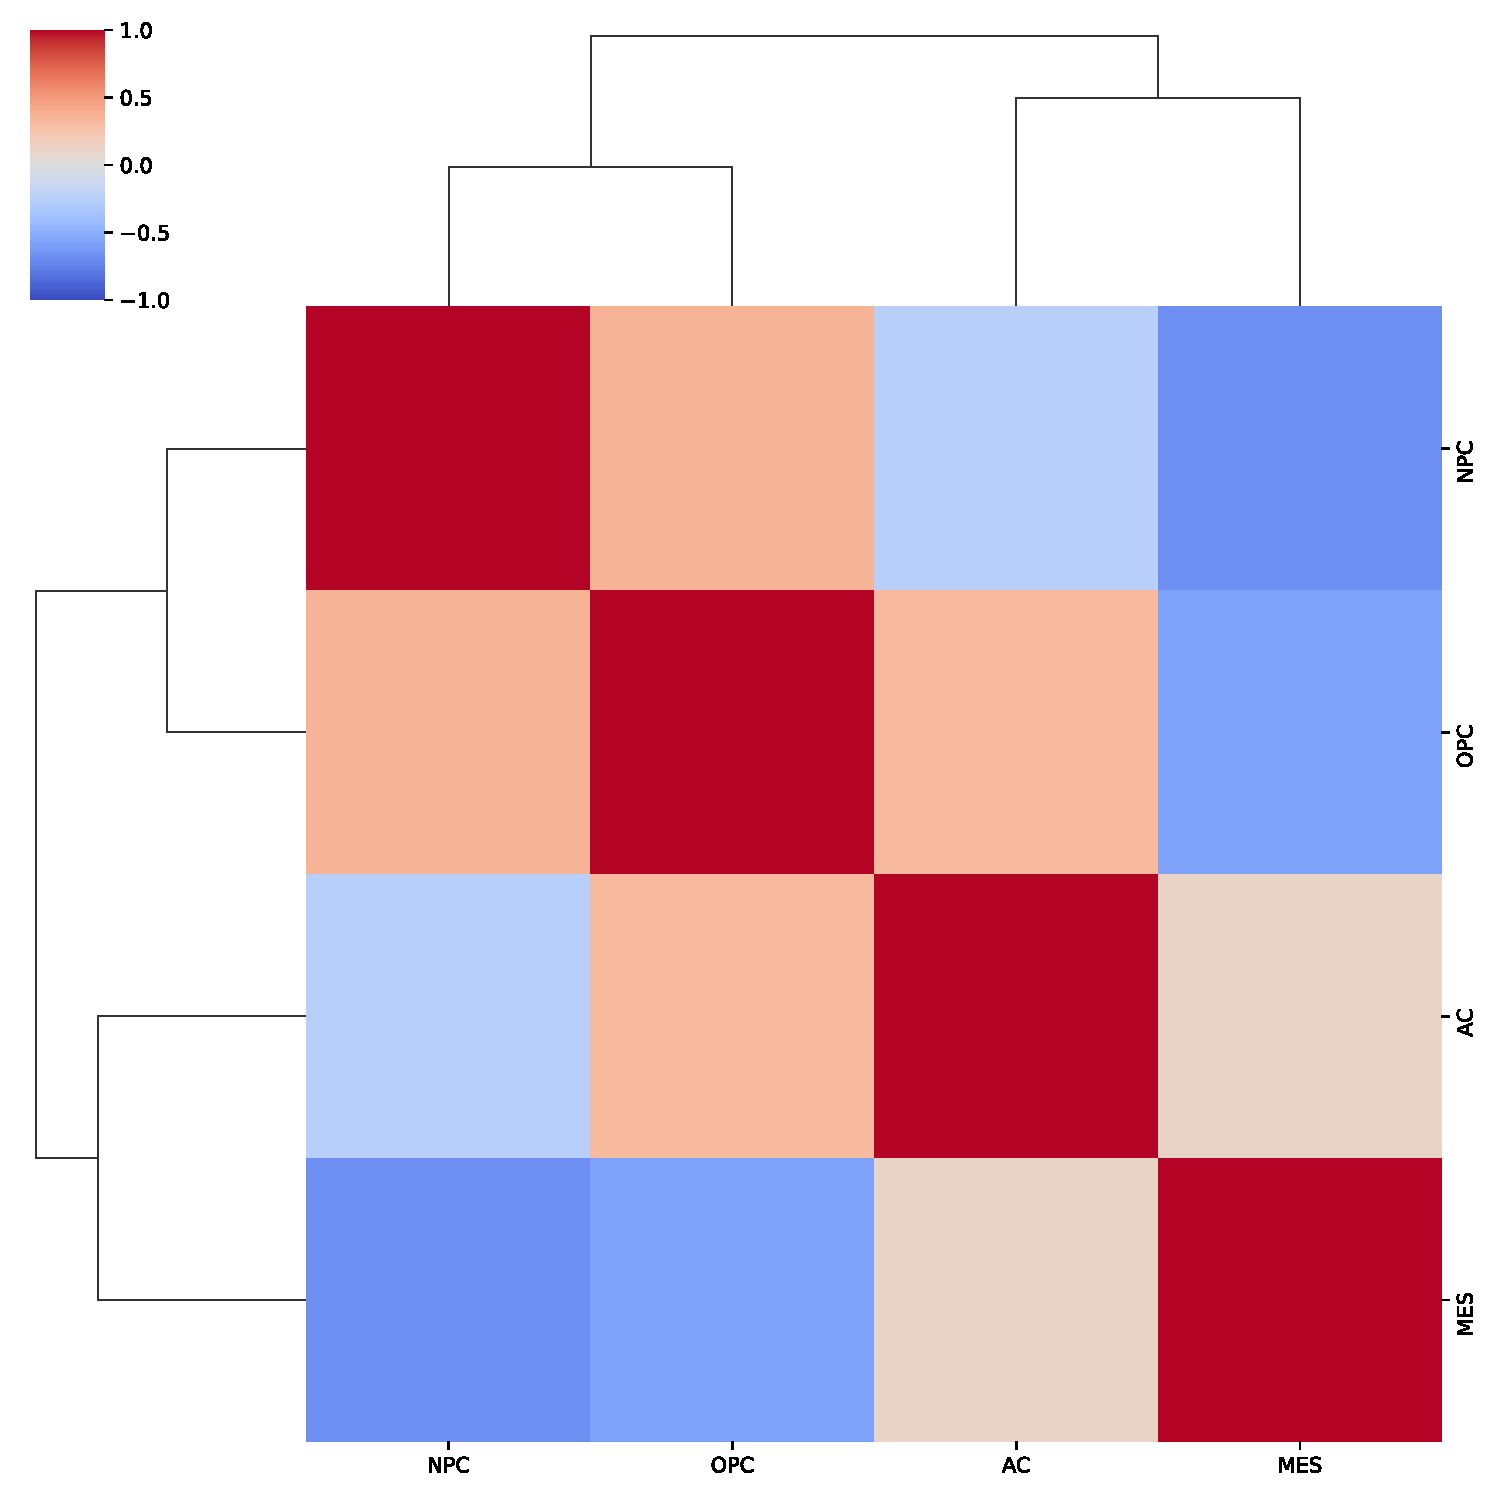
\includegraphics[width=\textwidth]{AUCell_GSM3828672_corrplot_4D}
                    \caption{GSE131928 - GSM3828672 (Smartseq2)}
                \end{subfigure}
                \begin{subfigure}[b]{0.38\textwidth}
                    \centering
                    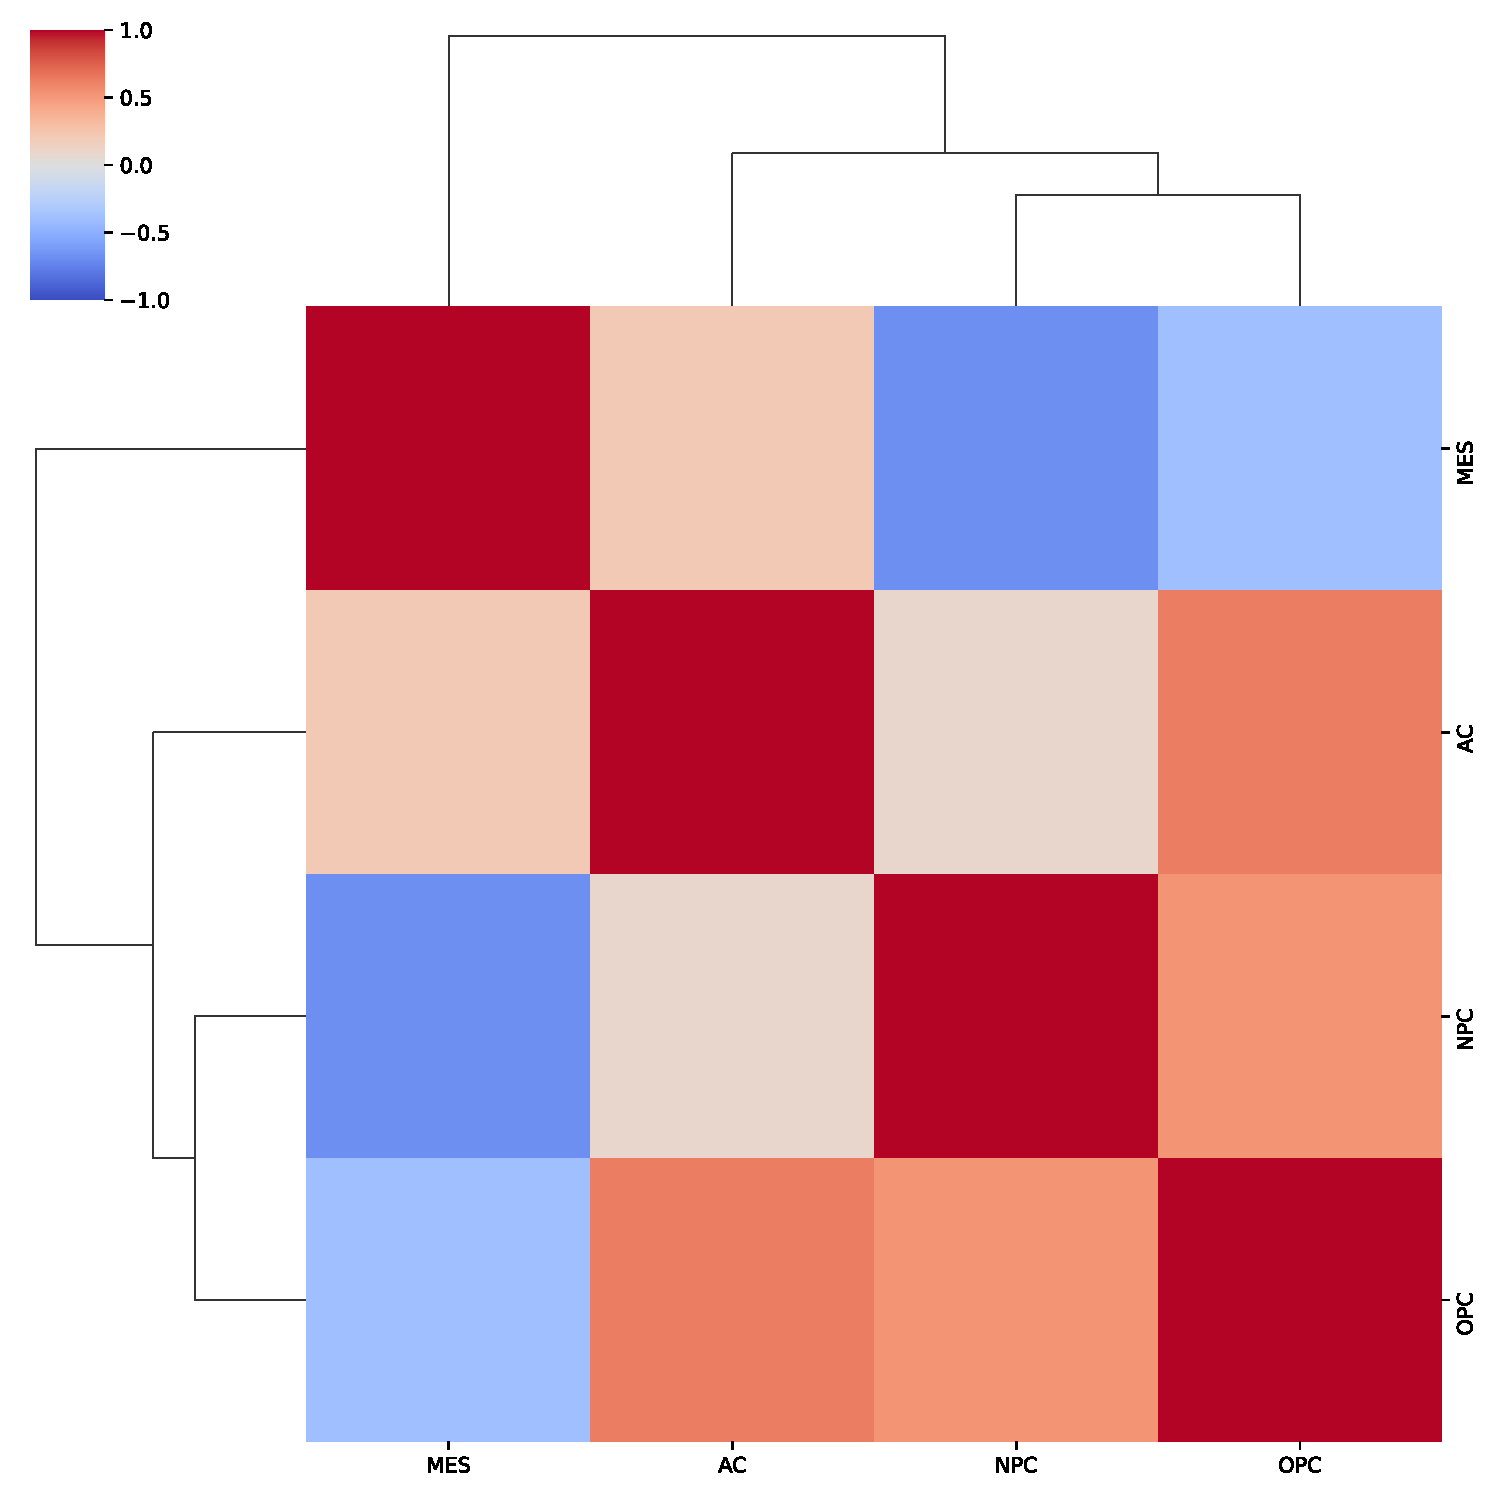
\includegraphics[width=\textwidth]{AUCell_GSM3828673_corrplot_4D}
                    \caption{GSE131928 - GSM3828673 (10X)}
                \end{subfigure}
                \caption{Correlation of ssGSEA/AUCell scores}
            \end{figure}
        \end{adjustwidth}
    \end{frame}

    \begin{frame}{ssGSEA/AUCell}
        \begin{adjustwidth}{-5cm}{-5cm}
            \centering
            \begin{figure}\ContinuedFloat
                \centering
                \begin{subfigure}[b]{0.38\textwidth}
                    \centering
                    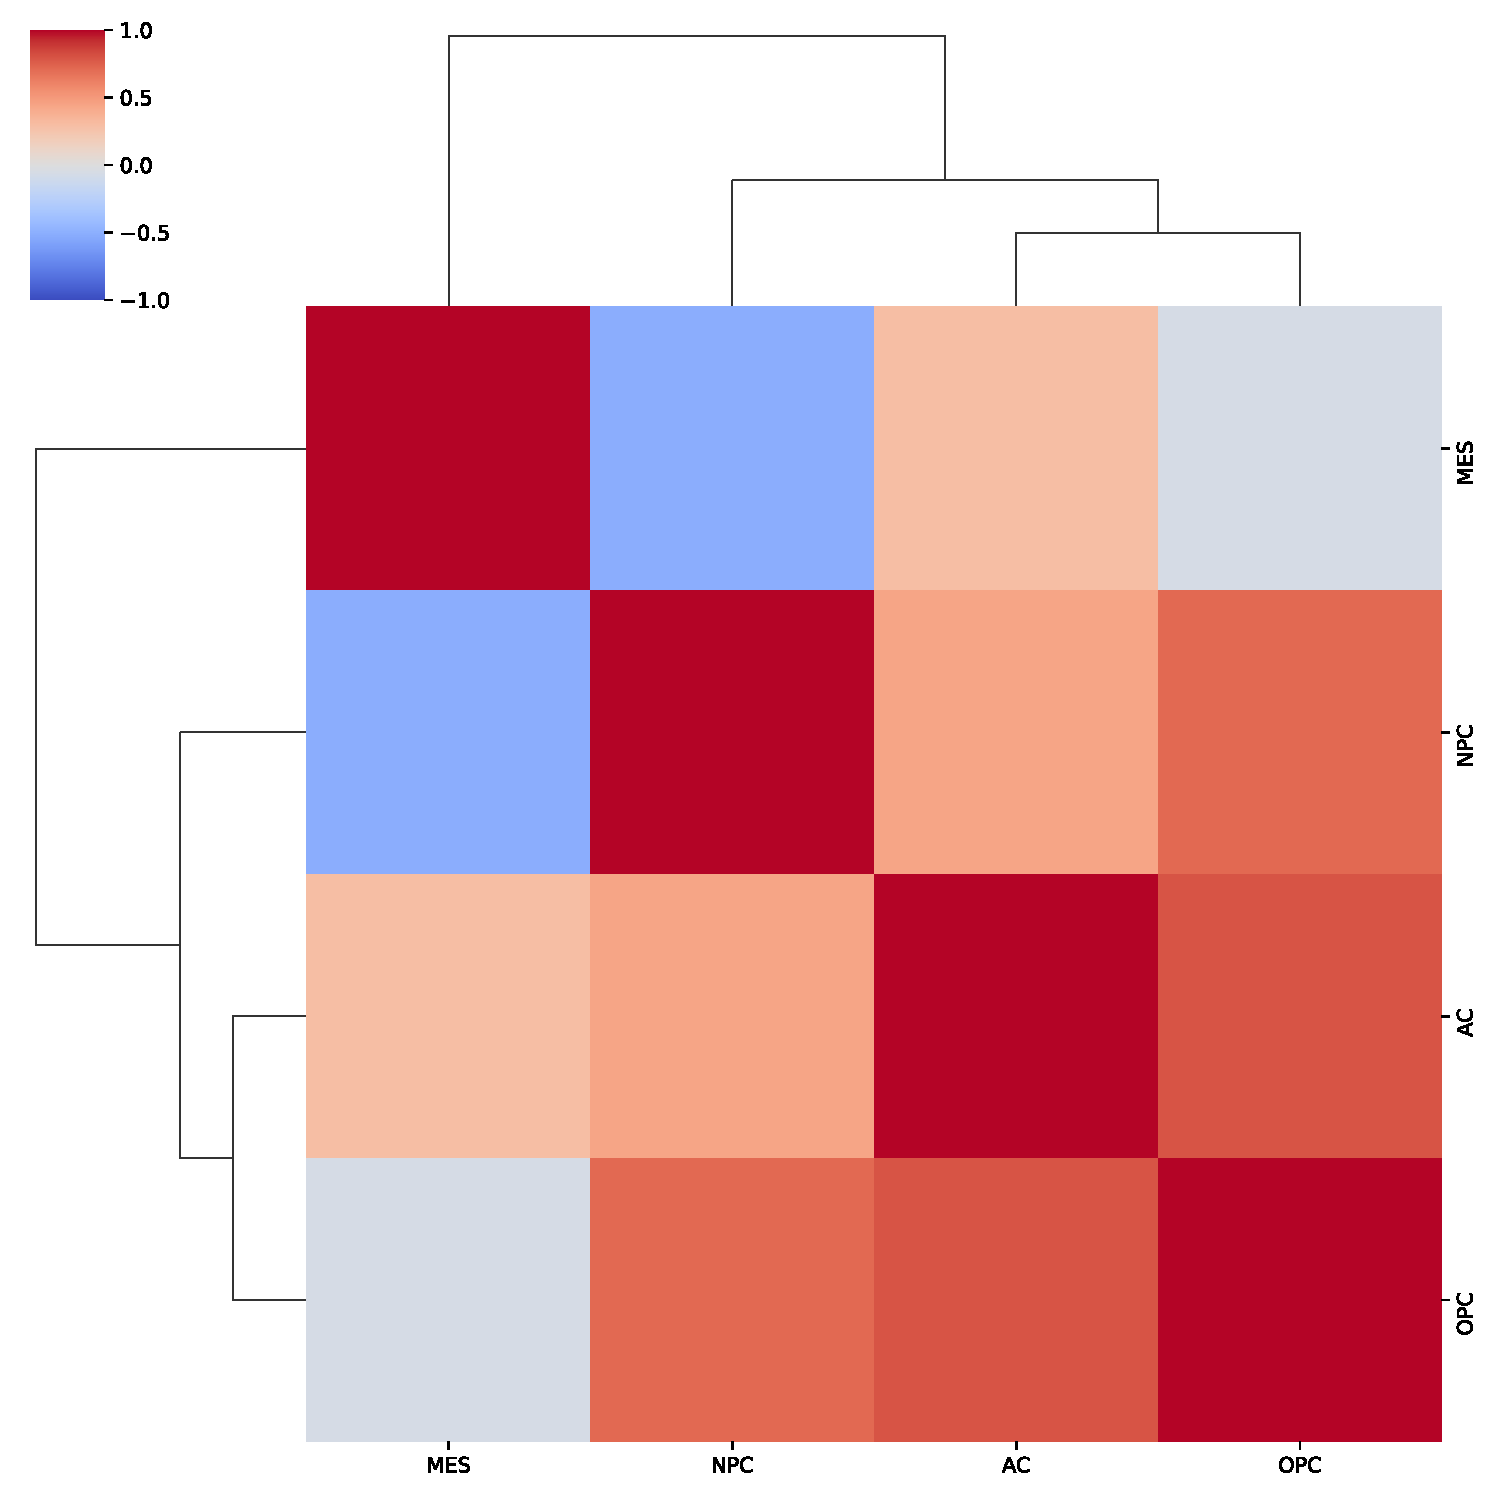
\includegraphics[width=\textwidth]{AUCell_OSM_celllines_corrplot_4D}
                    \caption{GSE168004 - OSM (treated)}
                \end{subfigure}
                \begin{subfigure}[b]{0.38\textwidth}
                    \centering
                    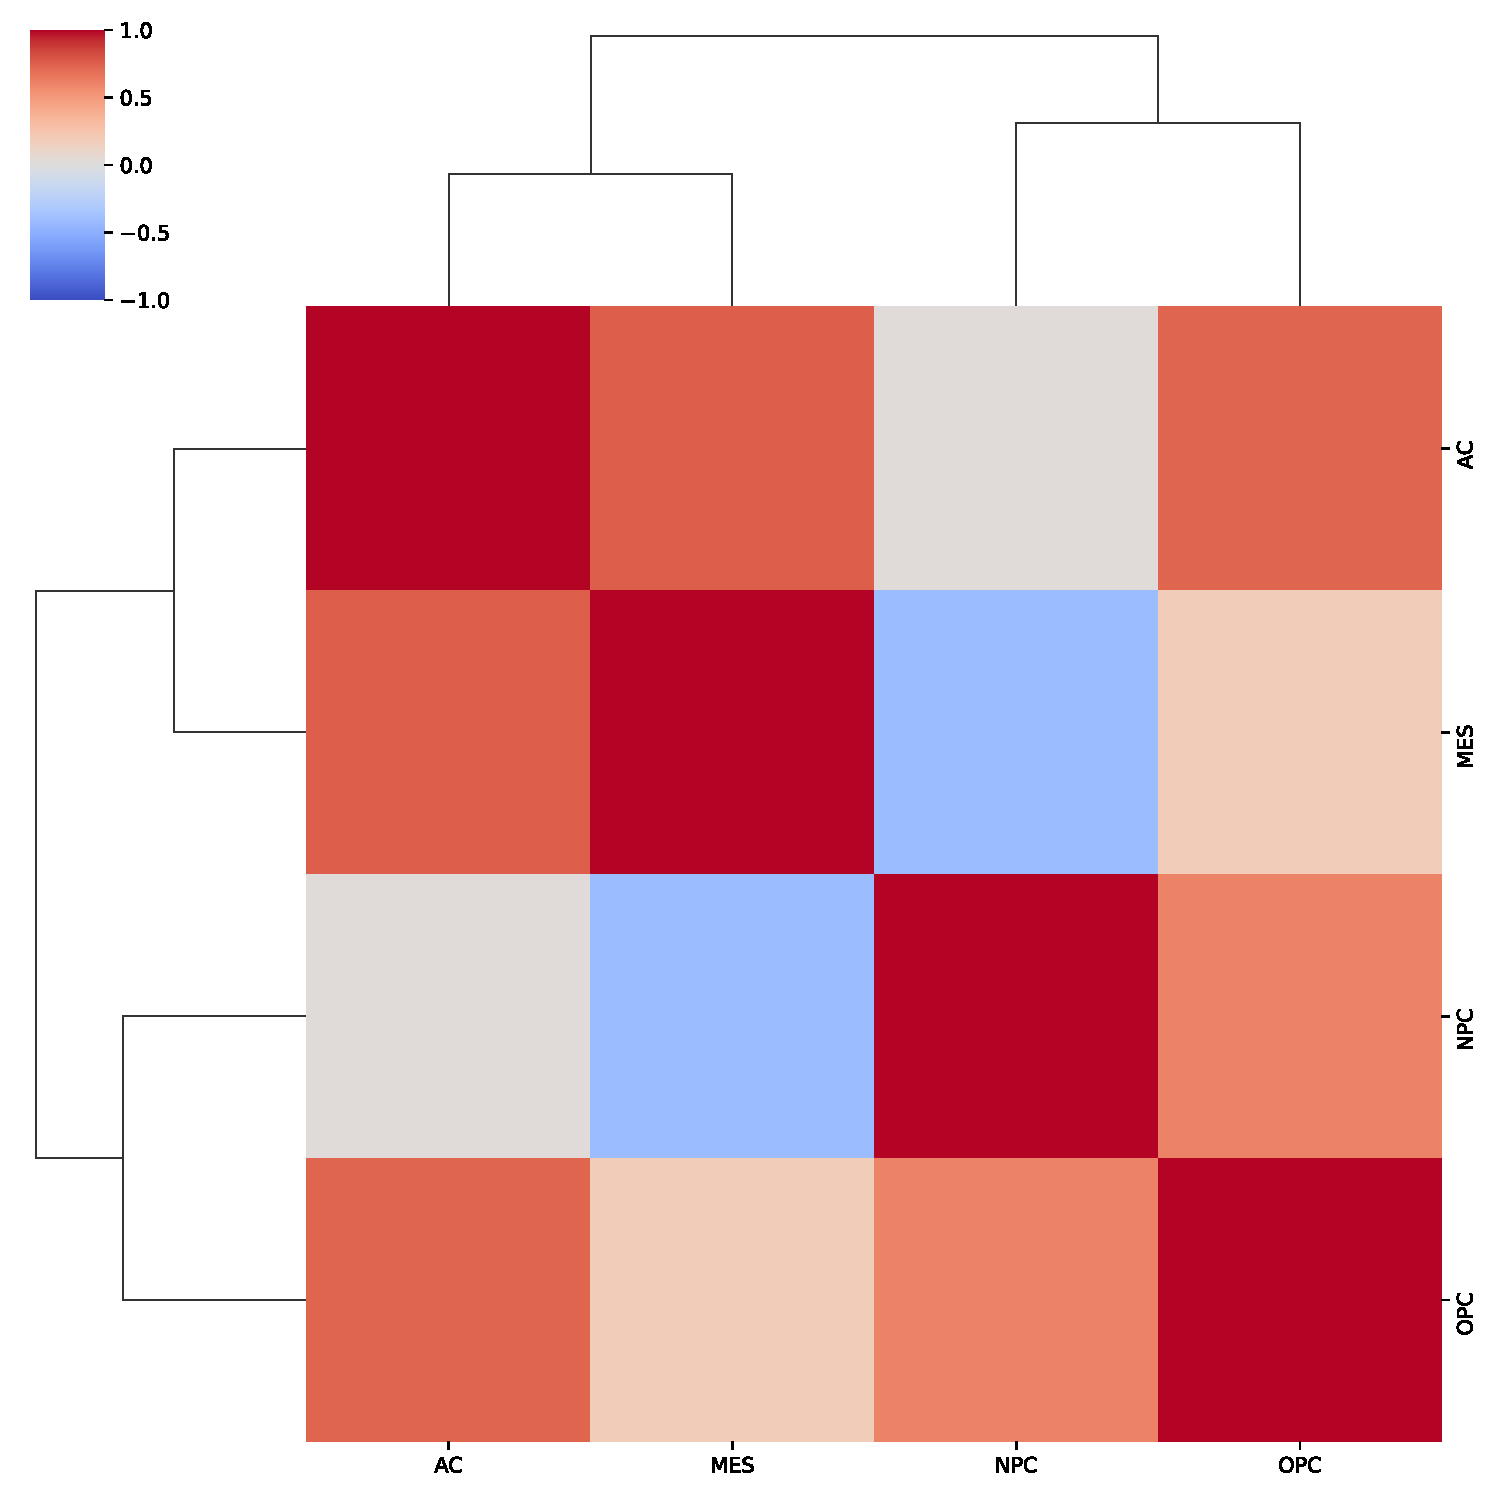
\includegraphics[width=\textwidth]{AUCell_mgg23_corrplot_4D}
                    \caption{GSE168004 - mgg23 (Control)}
                \end{subfigure}
                \begin{subfigure}[b]{0.38\textwidth}
                    \centering
                    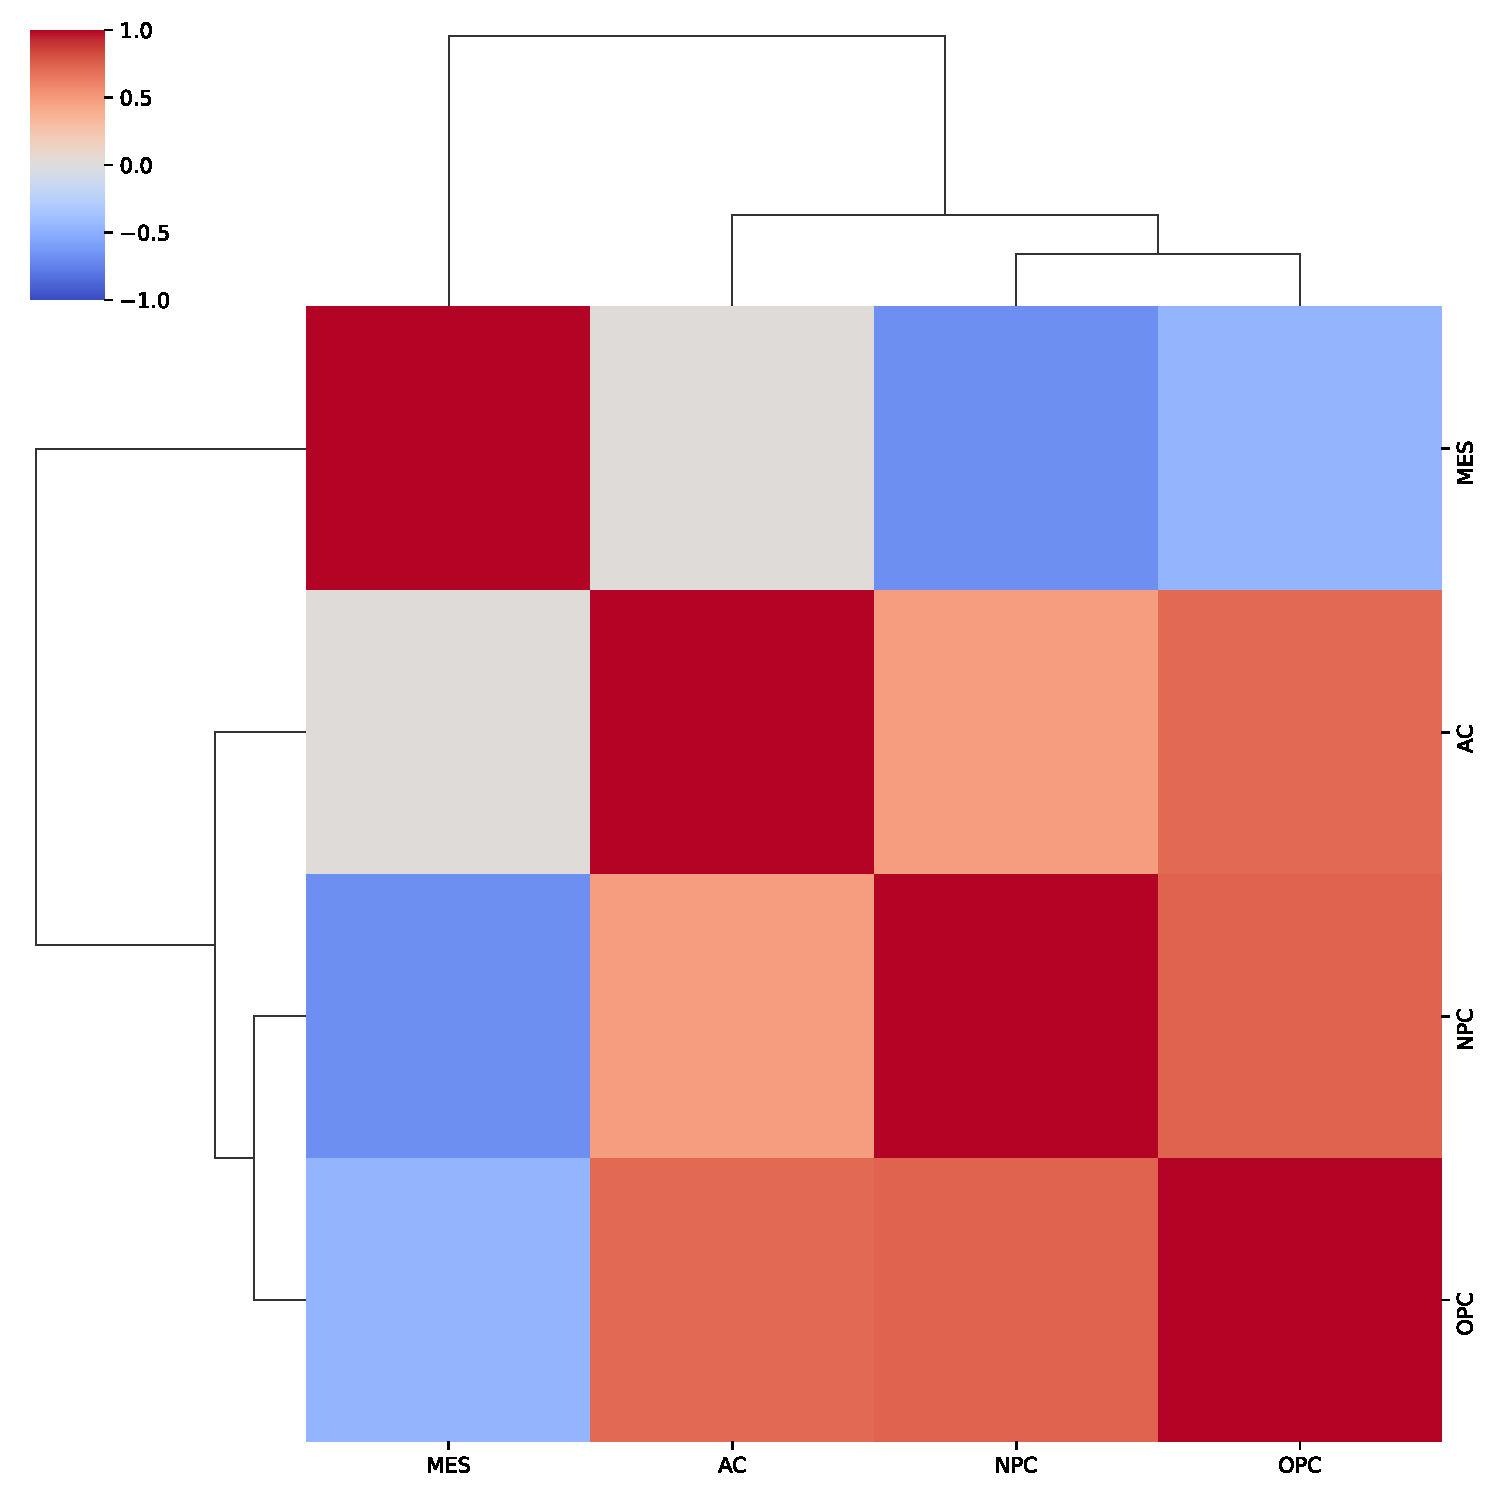
\includegraphics[width=\textwidth]{AUCell_mgg75_corrplot_4D}
                    \caption{GSE168004 - mgg75 (Control)}
                \end{subfigure}
                \caption{Correlation of ssGSEA/AUCell scores}
            \end{figure}
        \end{adjustwidth}
    \end{frame}

    \begin{frame}{Signature}
        \begin{figure}
            \centering
            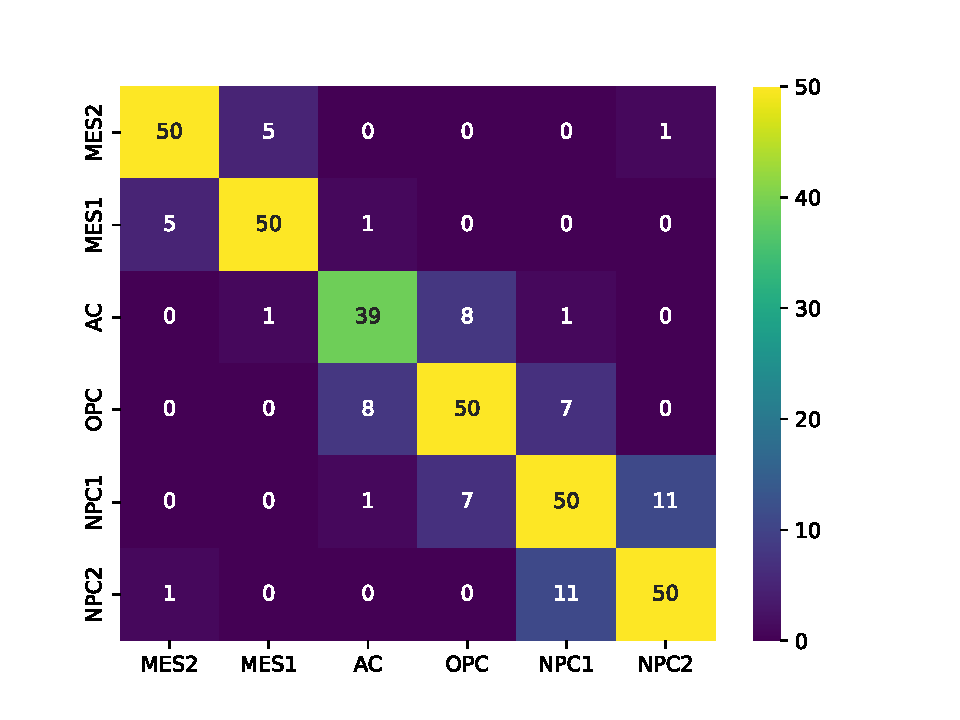
\includegraphics[width=0.6\textwidth]{signature_overlap}
            \caption{Overlap of genes in the signatures}
        \end{figure}
    \end{frame}

    \begin{frame}{Signature Expression Correlation}
        \begin{adjustwidth}{-5cm}{-5cm}
            \centering
            \begin{figure}
                \centering
                \begin{subfigure}[b]{0.38\textwidth}
                    \centering
                    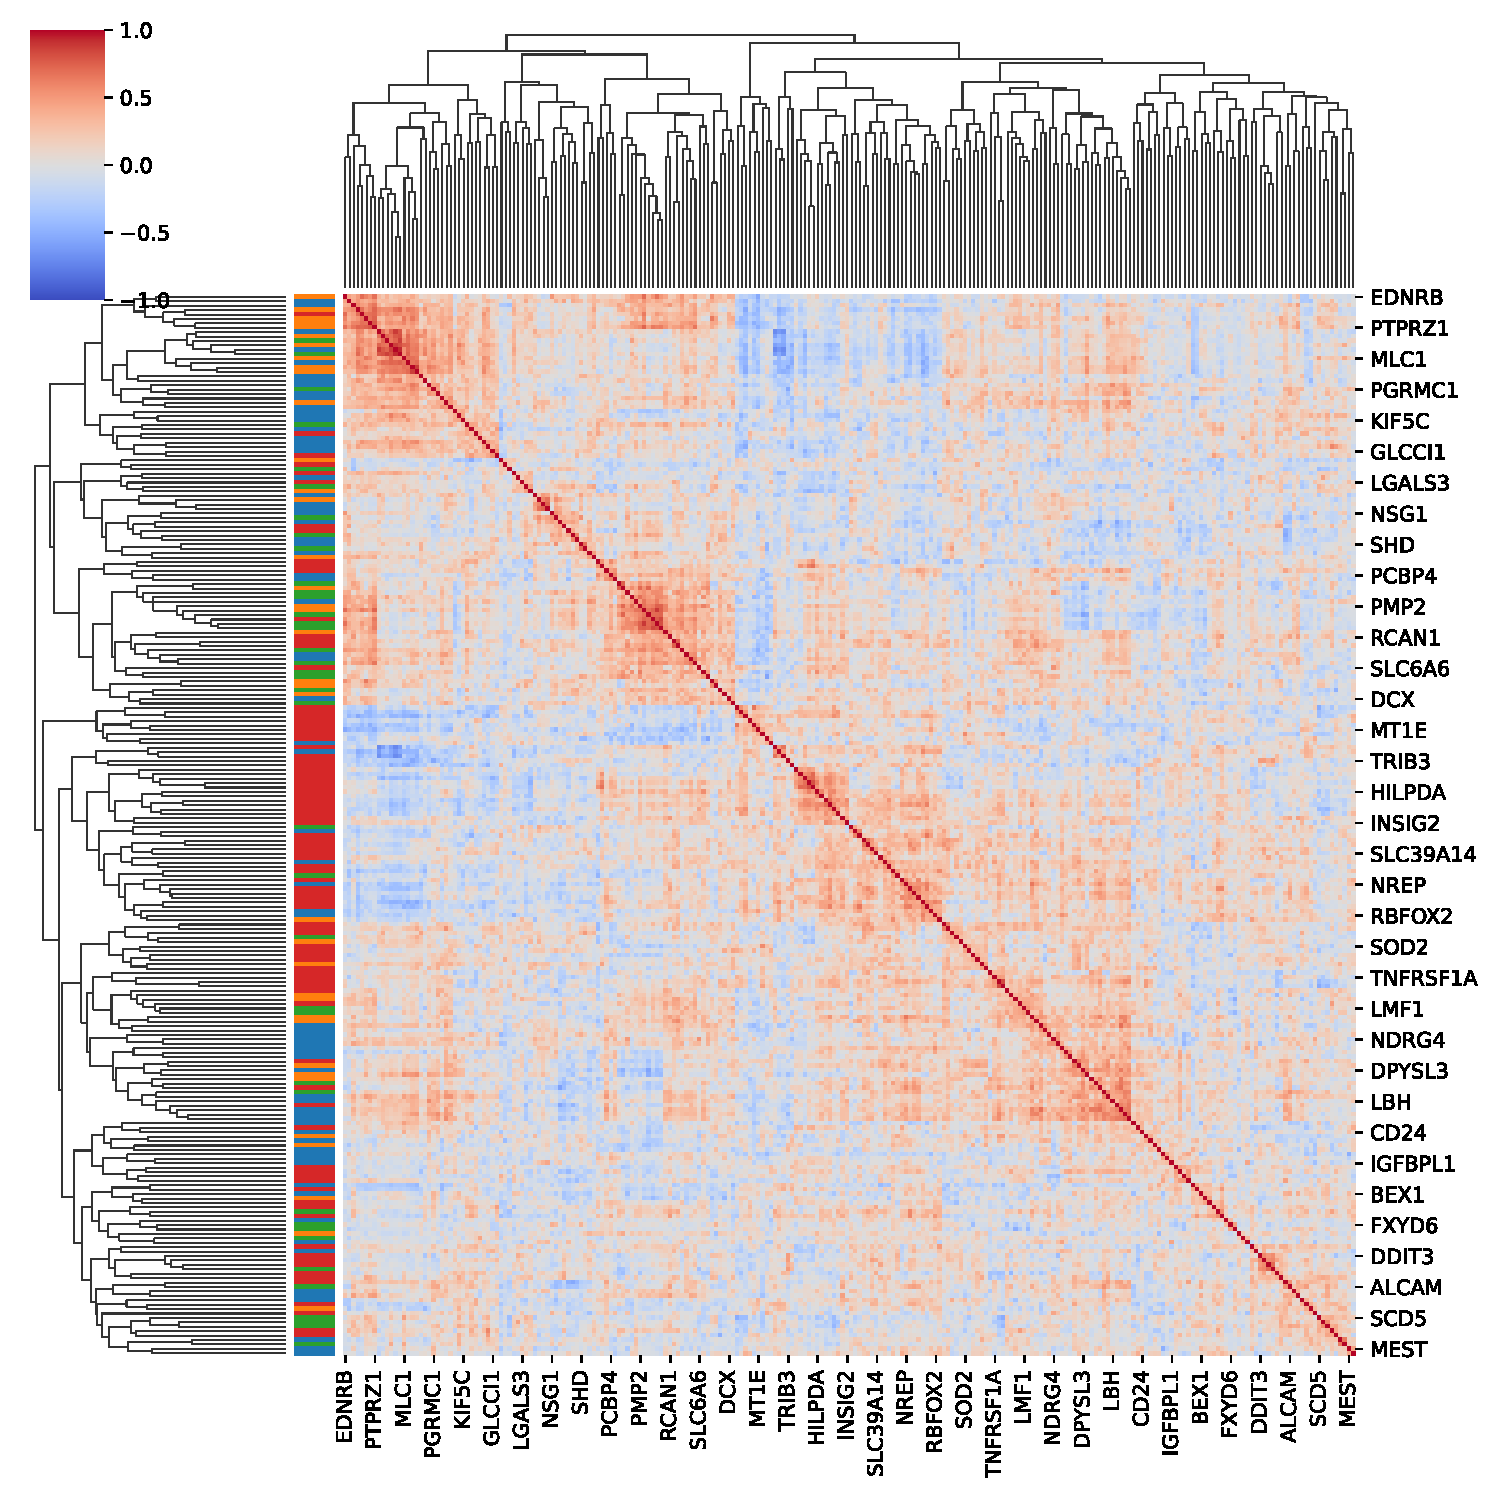
\includegraphics[width=\textwidth]{CCLE_Corrplot_coloured}
                    \caption{CCLE}
                \end{subfigure}
                \begin{subfigure}[b]{0.38\textwidth}
                    \centering
                    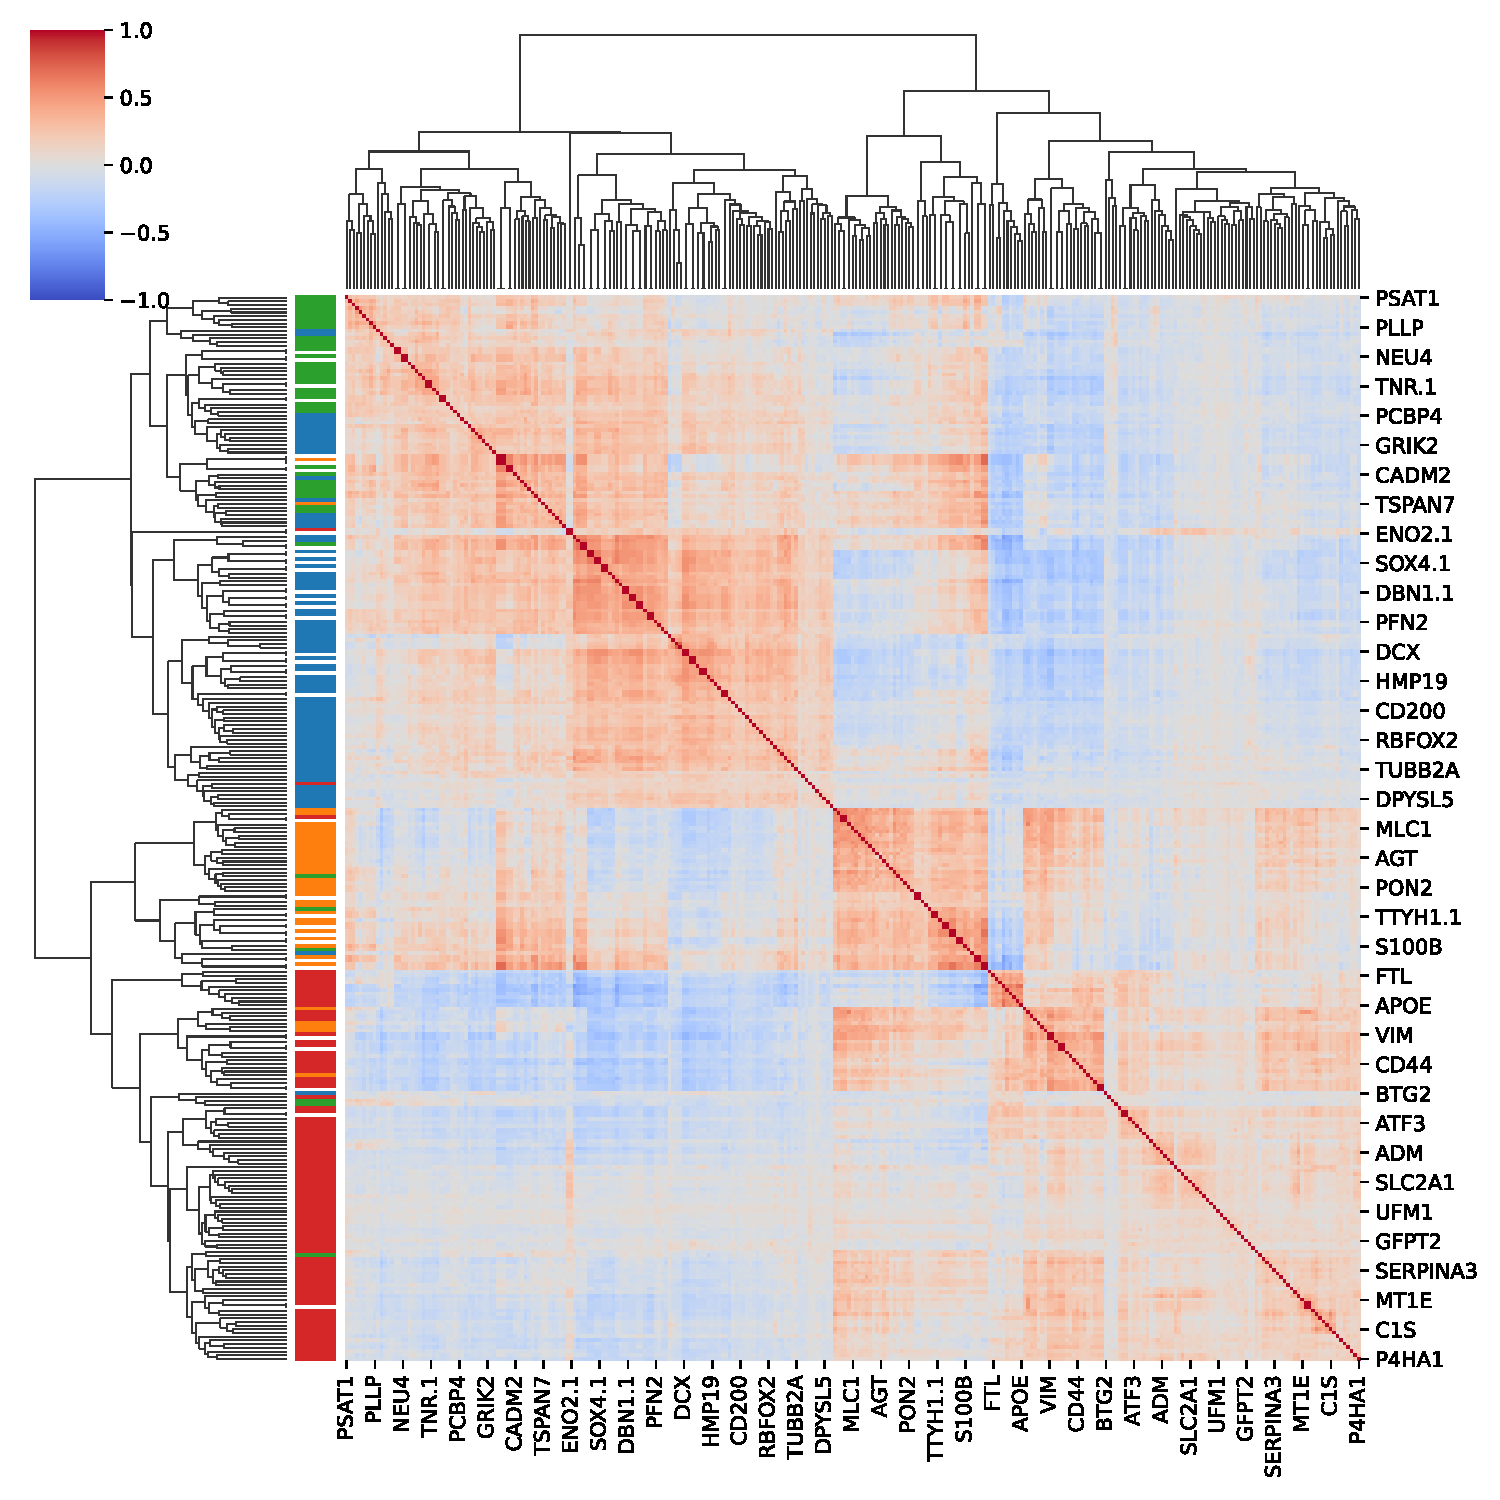
\includegraphics[width=\textwidth]{GSM3828672_Corrplot_coloured}
                    \caption{GSE131928 - GSM3828672 (Smartseq2)}
                \end{subfigure}
                \begin{subfigure}[b]{0.38\textwidth}
                    \centering
                    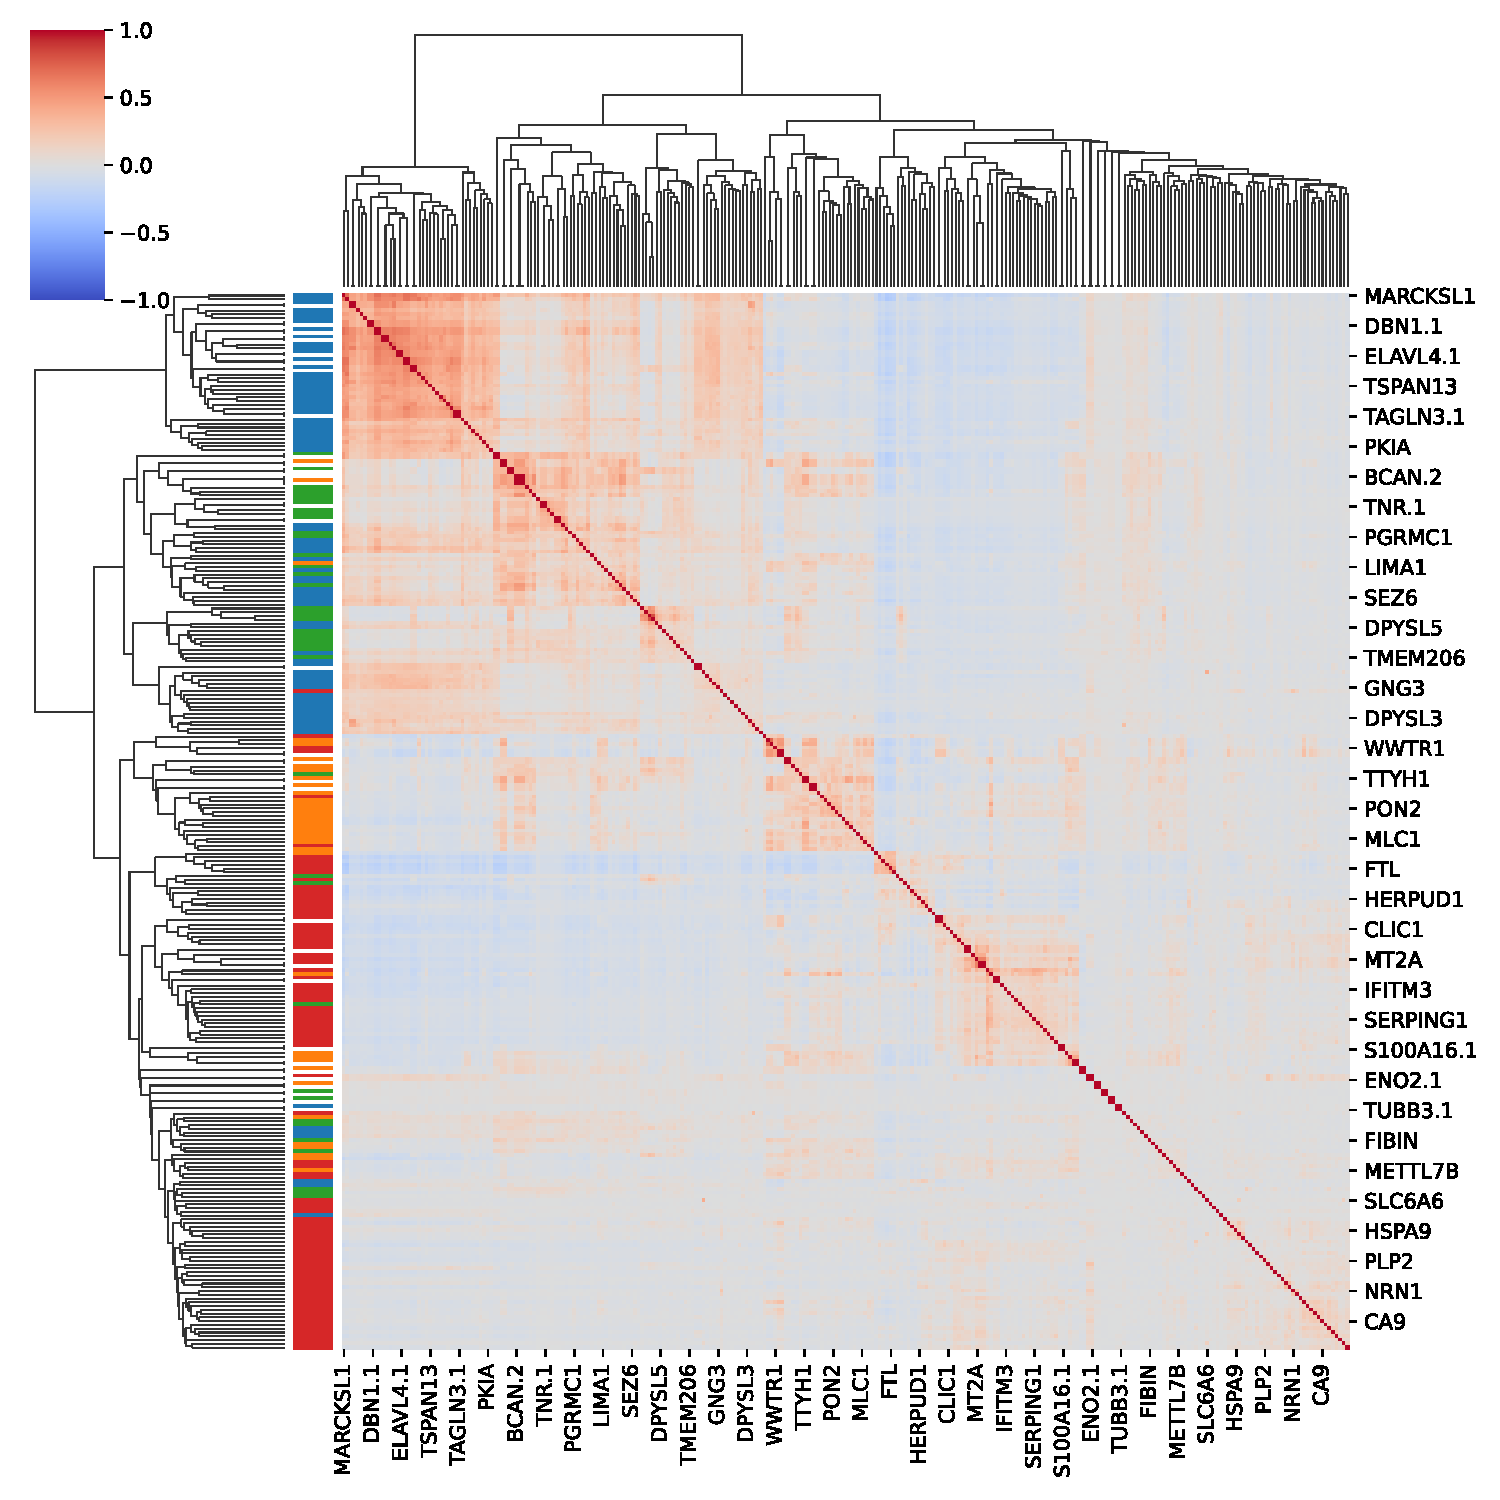
\includegraphics[width=\textwidth]{GSM3828673_Corrplot_coloured}
                    \caption{GSE131928 - GSM3828673 (10X)}
                \end{subfigure}
                \caption{Correlation of signature expression}
            \end{figure}
        \end{adjustwidth}
    \end{frame}

    \begin{frame}{Signature Expression Correlation}
        \begin{adjustwidth}{-5cm}{-5cm}
            \centering
            \begin{figure}\ContinuedFloat
                \centering
                \begin{subfigure}[b]{0.38\textwidth}
                    \centering
                    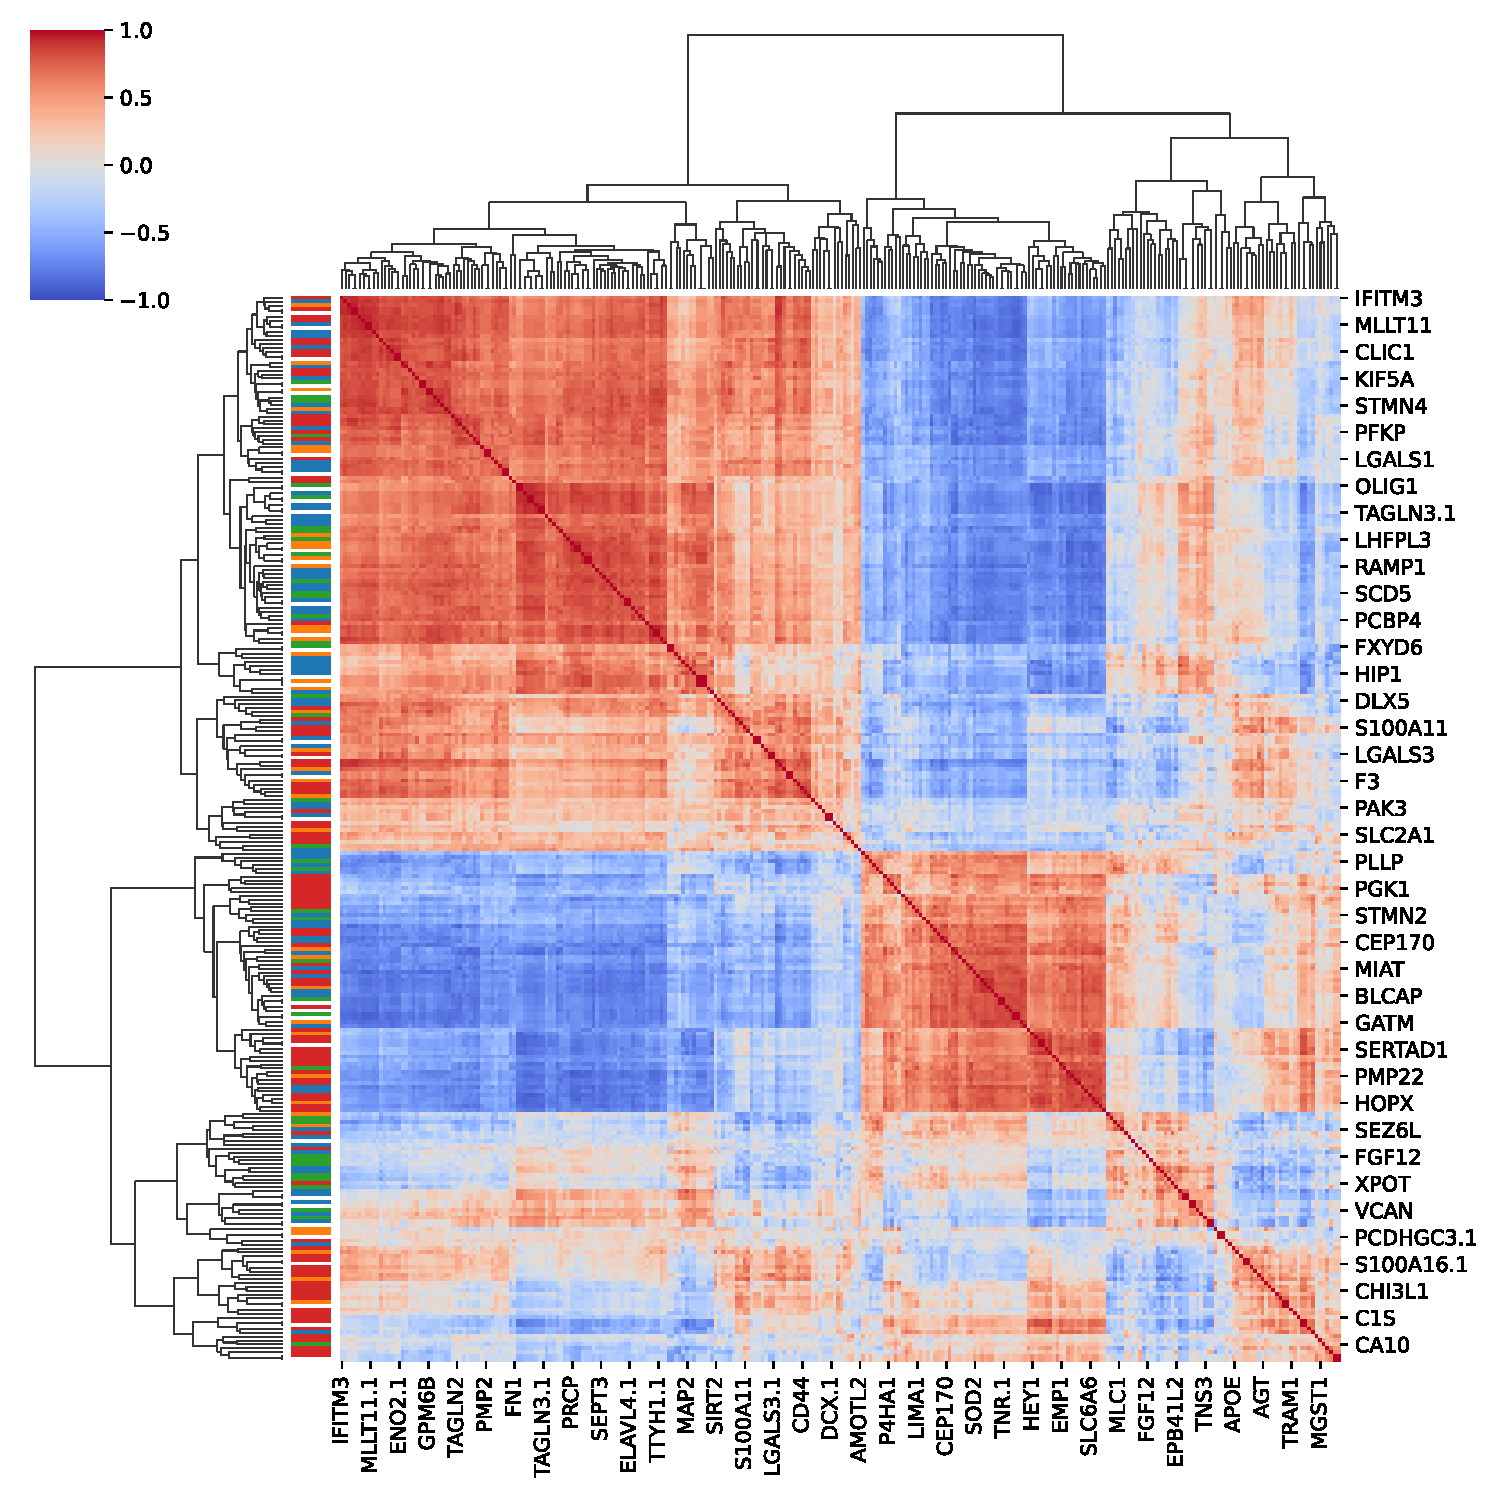
\includegraphics[width=\textwidth]{OSM_celllines_Corrplot_coloured}
                    \caption{GSE168004 - OSM (treated)}
                \end{subfigure}
                \begin{subfigure}[b]{0.38\textwidth}
                    \centering
                    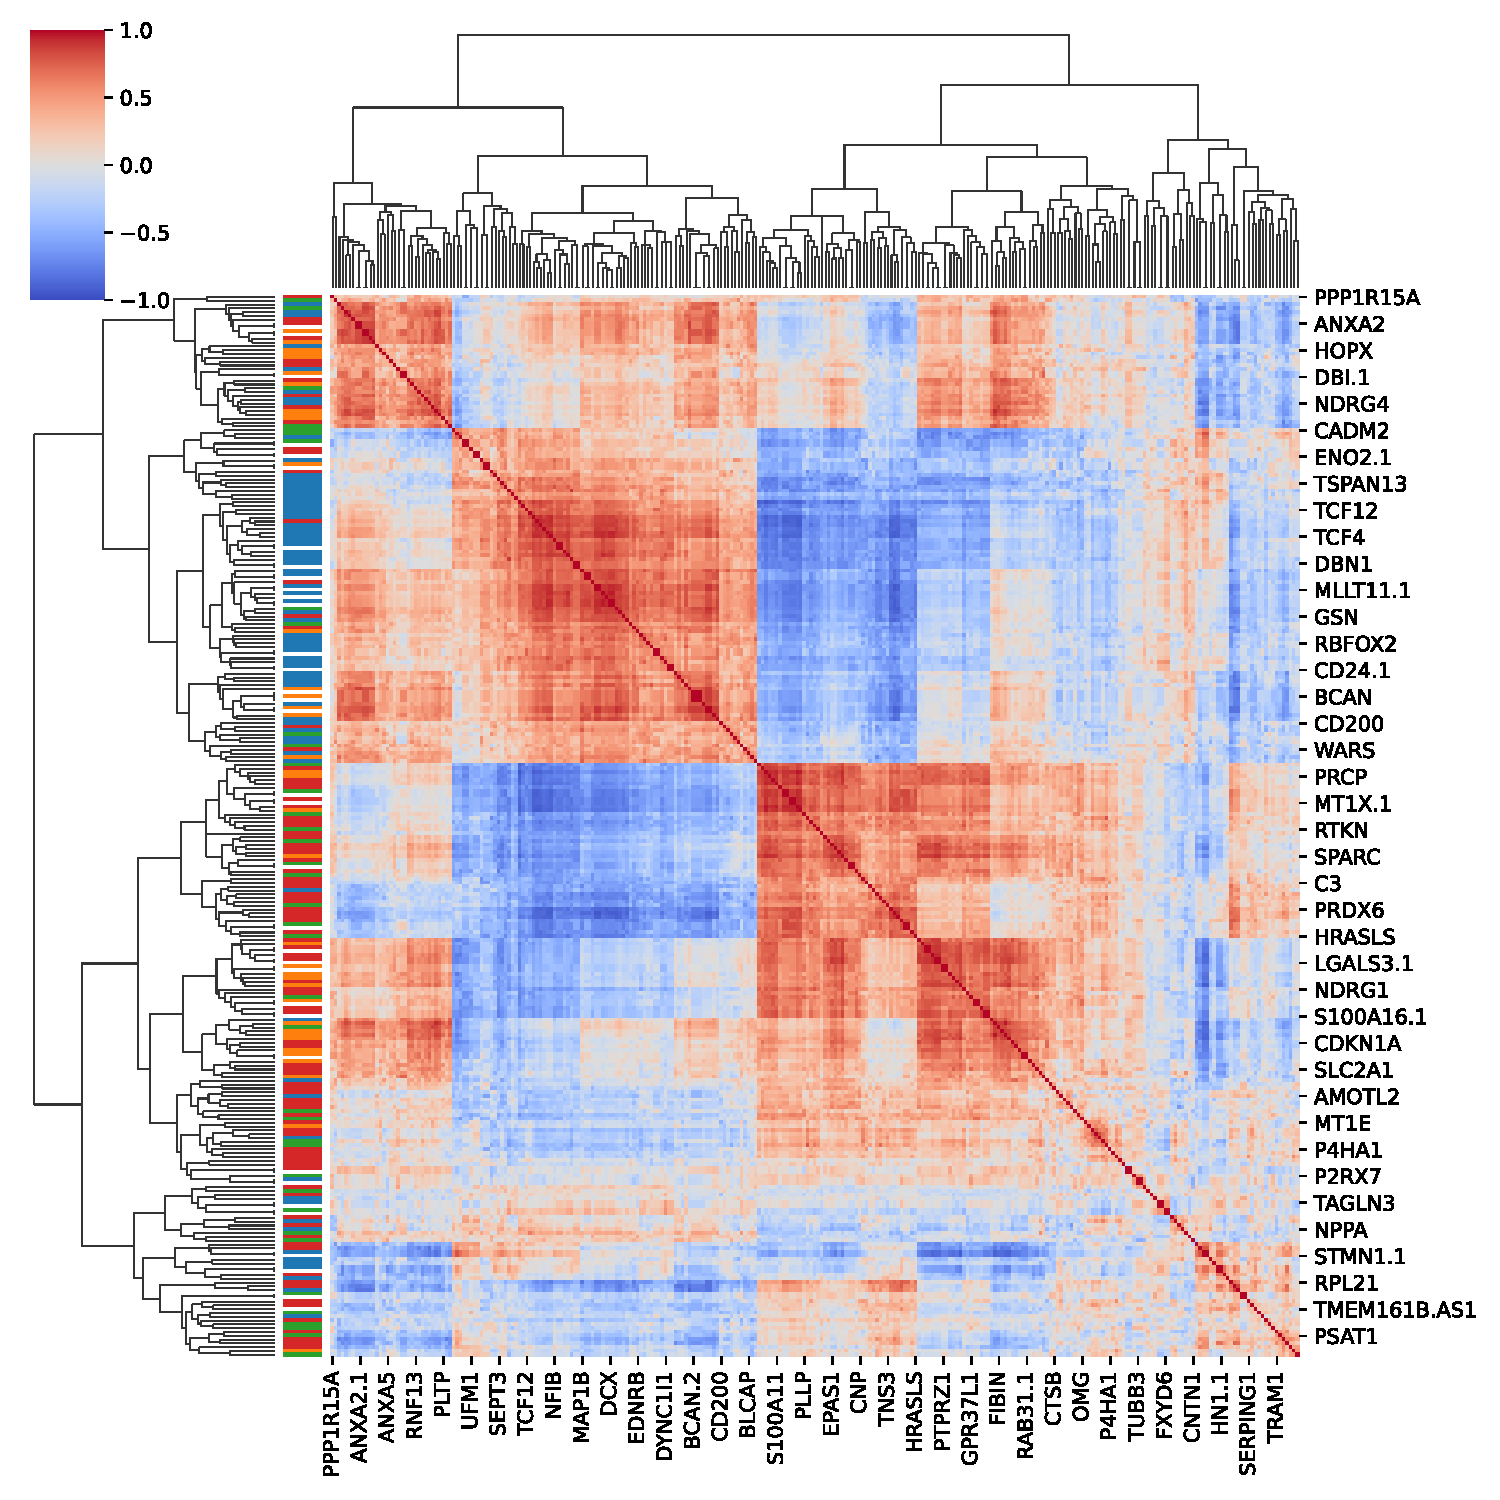
\includegraphics[width=\textwidth]{mgg23_Corrplot_coloured}
                    \caption{GSE168004 - mgg23 (Control)}
                \end{subfigure}
                \begin{subfigure}[b]{0.38\textwidth}
                    \centering
                    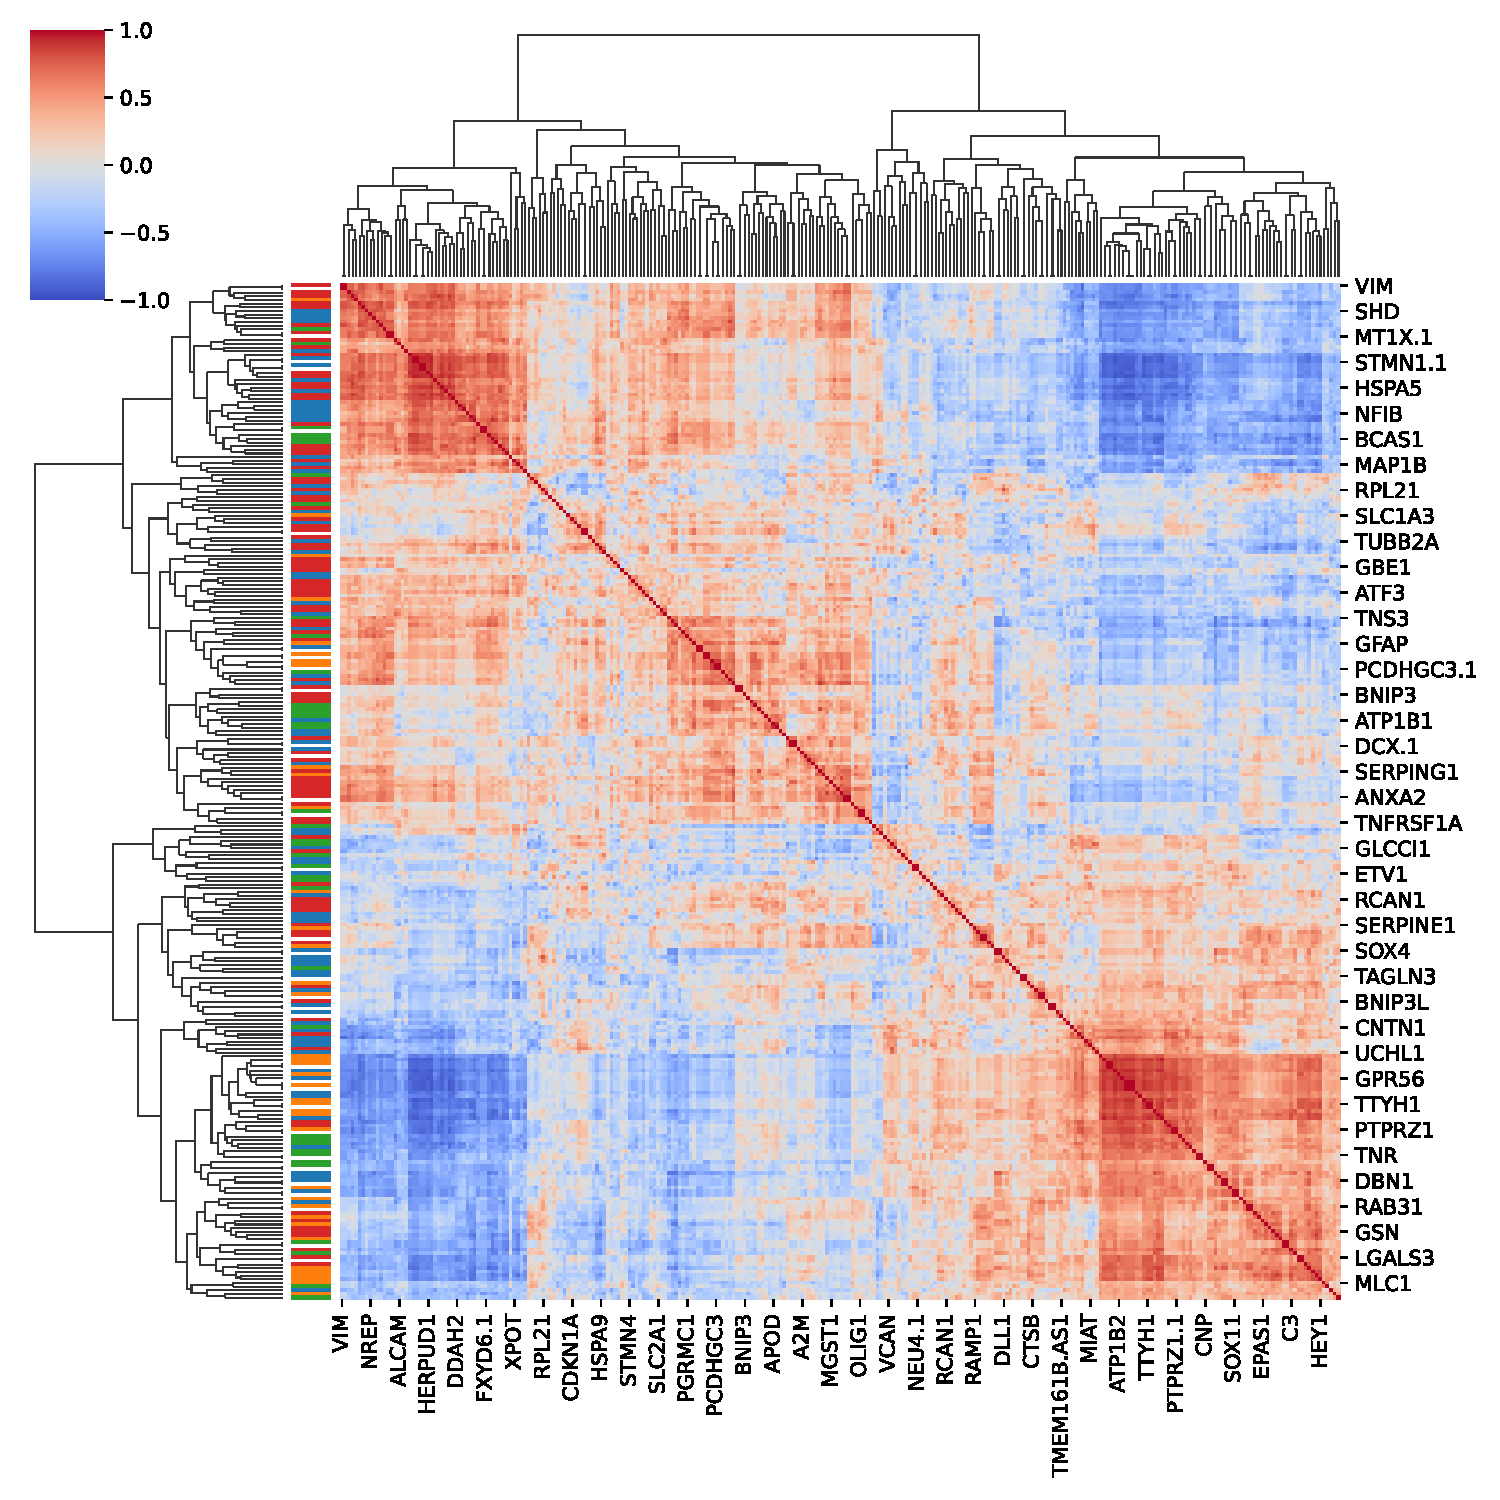
\includegraphics[width=\textwidth]{mgg75_Corrplot_coloured}
                    \caption{GSE168004 - mgg75 (Control)}
                \end{subfigure}
                \caption{Correlation of signature expression}
            \end{figure}
        \end{adjustwidth}
    \end{frame}

    \begin{frame}{Signature Expression Correlation Consistency}
        \begin{adjustwidth}{-5cm}{-5cm}
            \centering
            \begin{figure}
                \centering
                \begin{subfigure}[b]{0.38\textwidth}
                    \centering
                    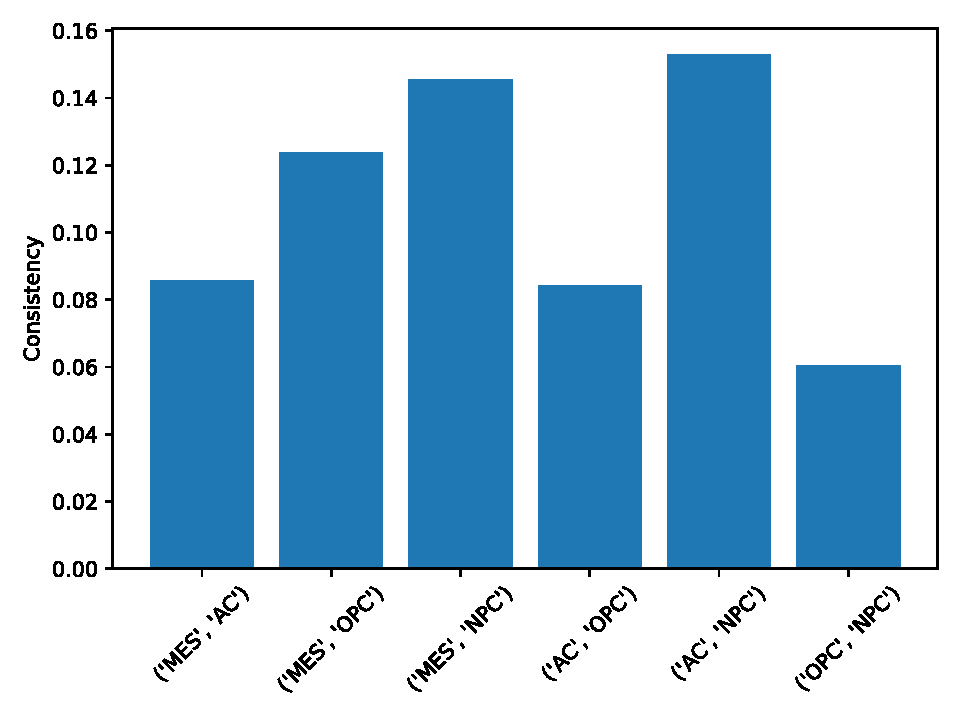
\includegraphics[width=\textwidth]{GSM3828672_Consistency}
                    \caption{GSE131928 - GSM3828672 (Smartseq2)}
                \end{subfigure}
                \begin{subfigure}[b]{0.38\textwidth}
                    \centering
                    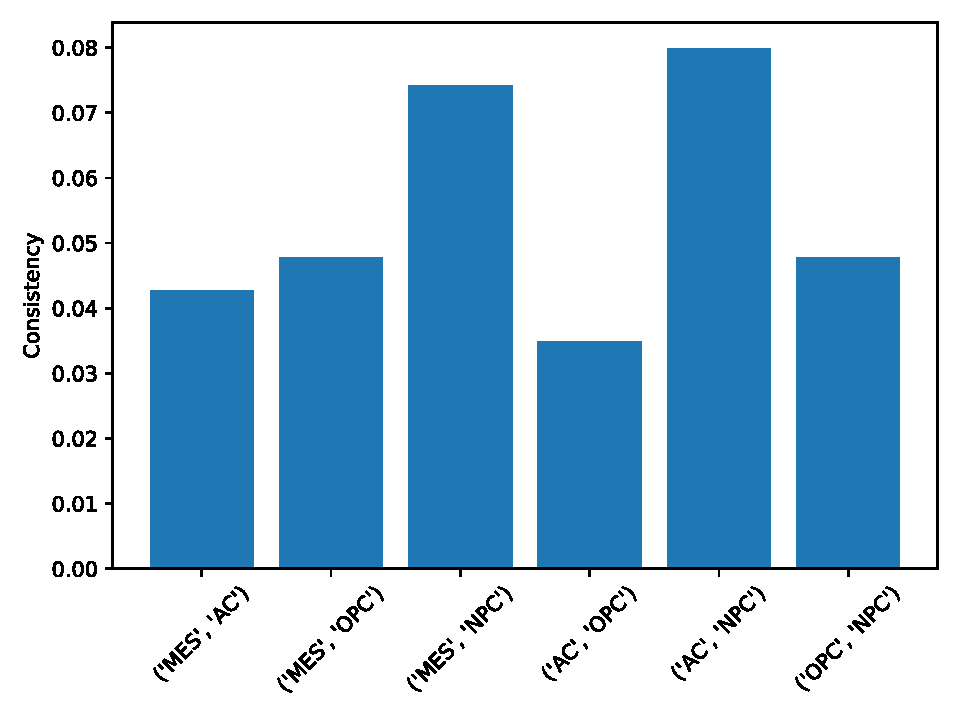
\includegraphics[width=\textwidth]{GSM3828673_Consistency}
                    \caption{GSE131928 - GSM3828673 (10X)}
                \end{subfigure}
                \caption{Consistency of correlation of signature expression}
            \end{figure}
        \end{adjustwidth}
    \end{frame}

    \begin{frame}{Signature Expression Correlation Consistency}
        \begin{adjustwidth}{-5cm}{-5cm}
            \centering
            \begin{figure}\ContinuedFloat
                \centering
                \begin{subfigure}[b]{0.38\textwidth}
                    \centering
                    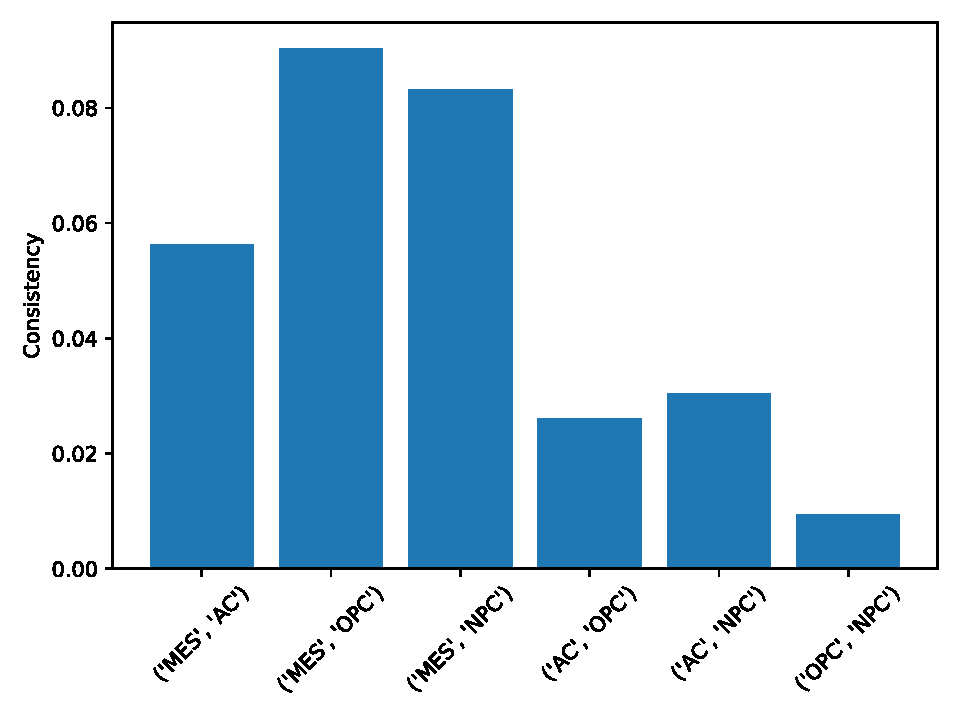
\includegraphics[width=\textwidth]{OSM_celllines_Consistency}
                    \caption{GSE168004 - OSM (treated)}
                \end{subfigure}
                \begin{subfigure}[b]{0.38\textwidth}
                    \centering
                    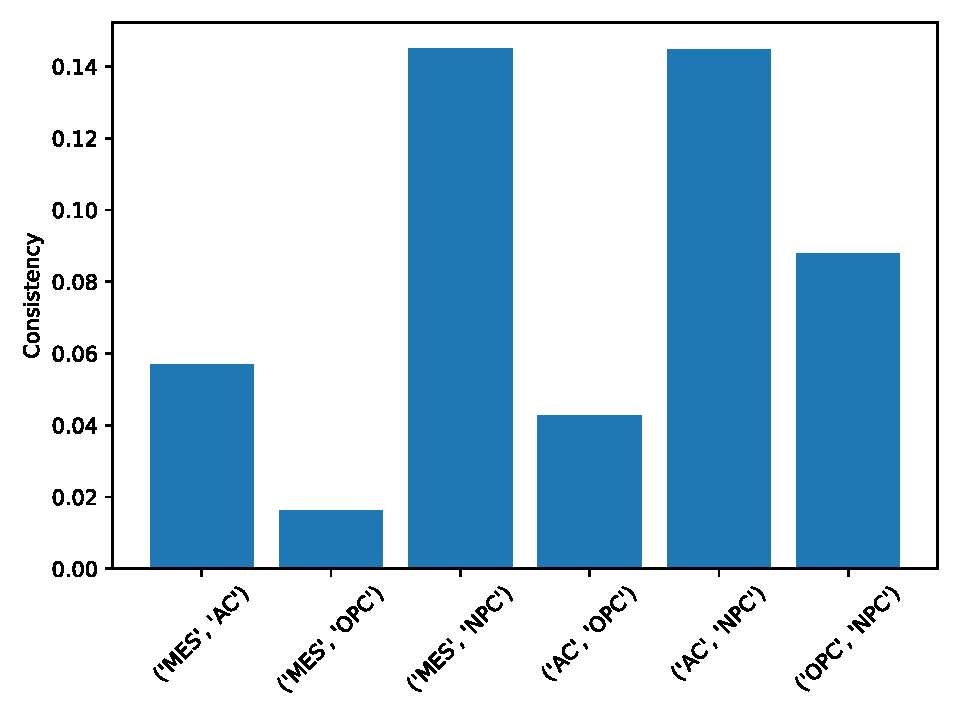
\includegraphics[width=\textwidth]{mgg23_Consistency}
                    \caption{GSE168004 - mgg23 (Control)}
                \end{subfigure}
                \begin{subfigure}[b]{0.38\textwidth}
                    \centering
                    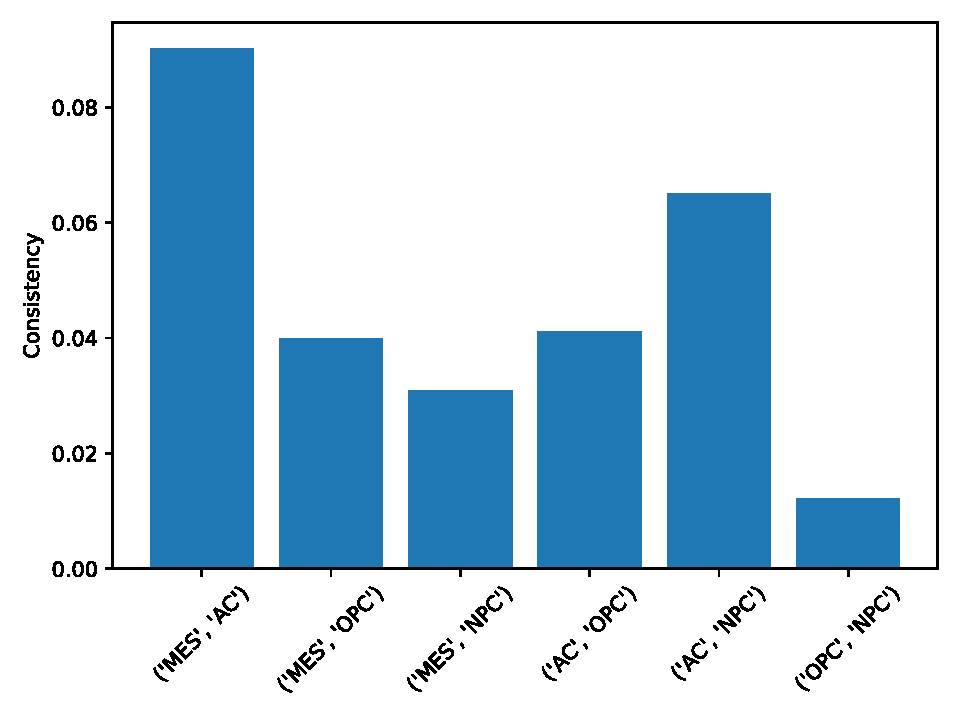
\includegraphics[width=\textwidth]{mgg75_Consistency}
                    \caption{GSE168004 - mgg75 (Control)}
                \end{subfigure}
                \caption{Consistency of correlation of signature expression}
            \end{figure}
        \end{adjustwidth}
    \end{frame}

    \begin{frame}{Signature PCA}
        \begin{adjustwidth}{-5cm}{-5cm}
            \centering
            \begin{figure}
                \centering
                \begin{subfigure}[b]{0.38\textwidth}
                    \centering
                    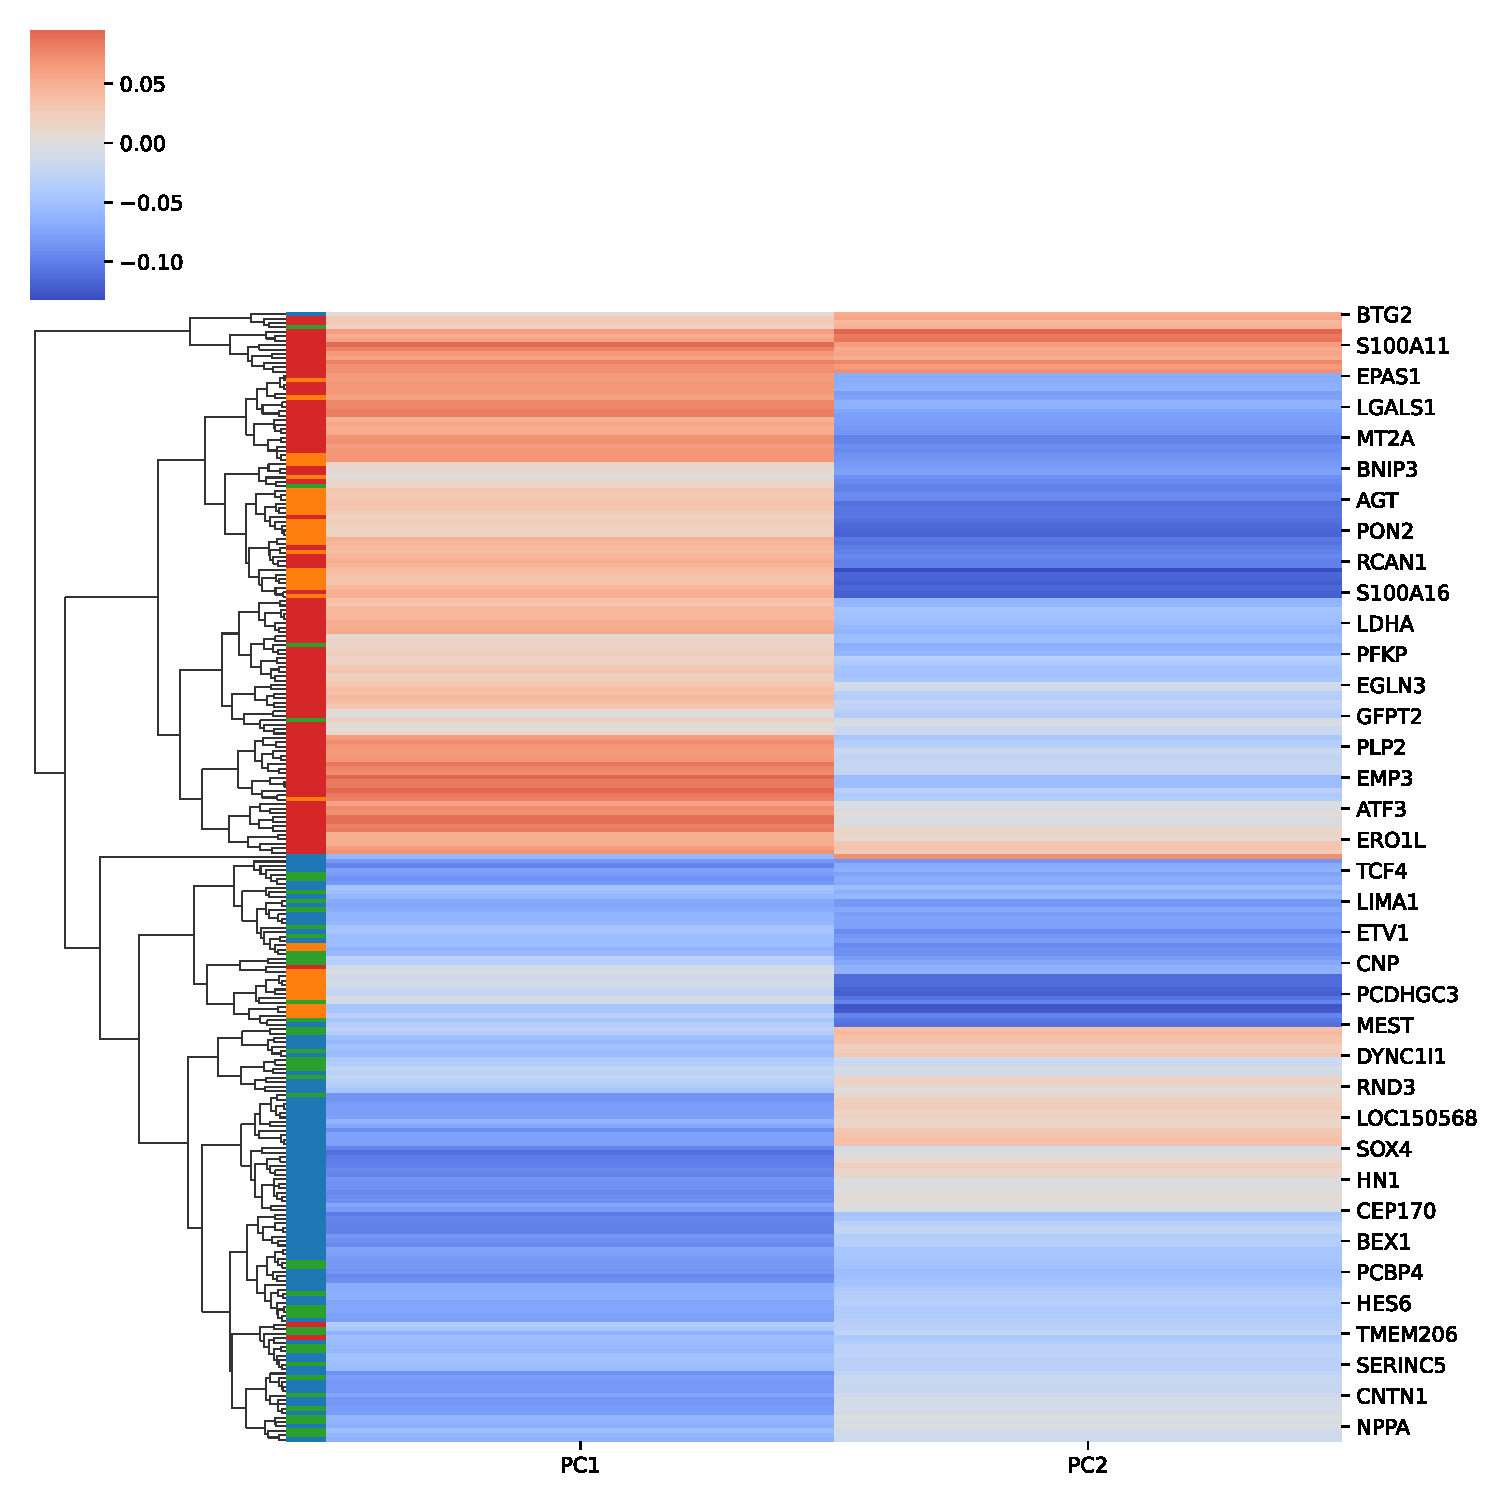
\includegraphics[width=\textwidth]{GSM3828672_loadings_plot}
                    \caption{GSE131928 - GSM3828672 (Smartseq2)}
                \end{subfigure}
                \begin{subfigure}[b]{0.38\textwidth}
                    \centering
                    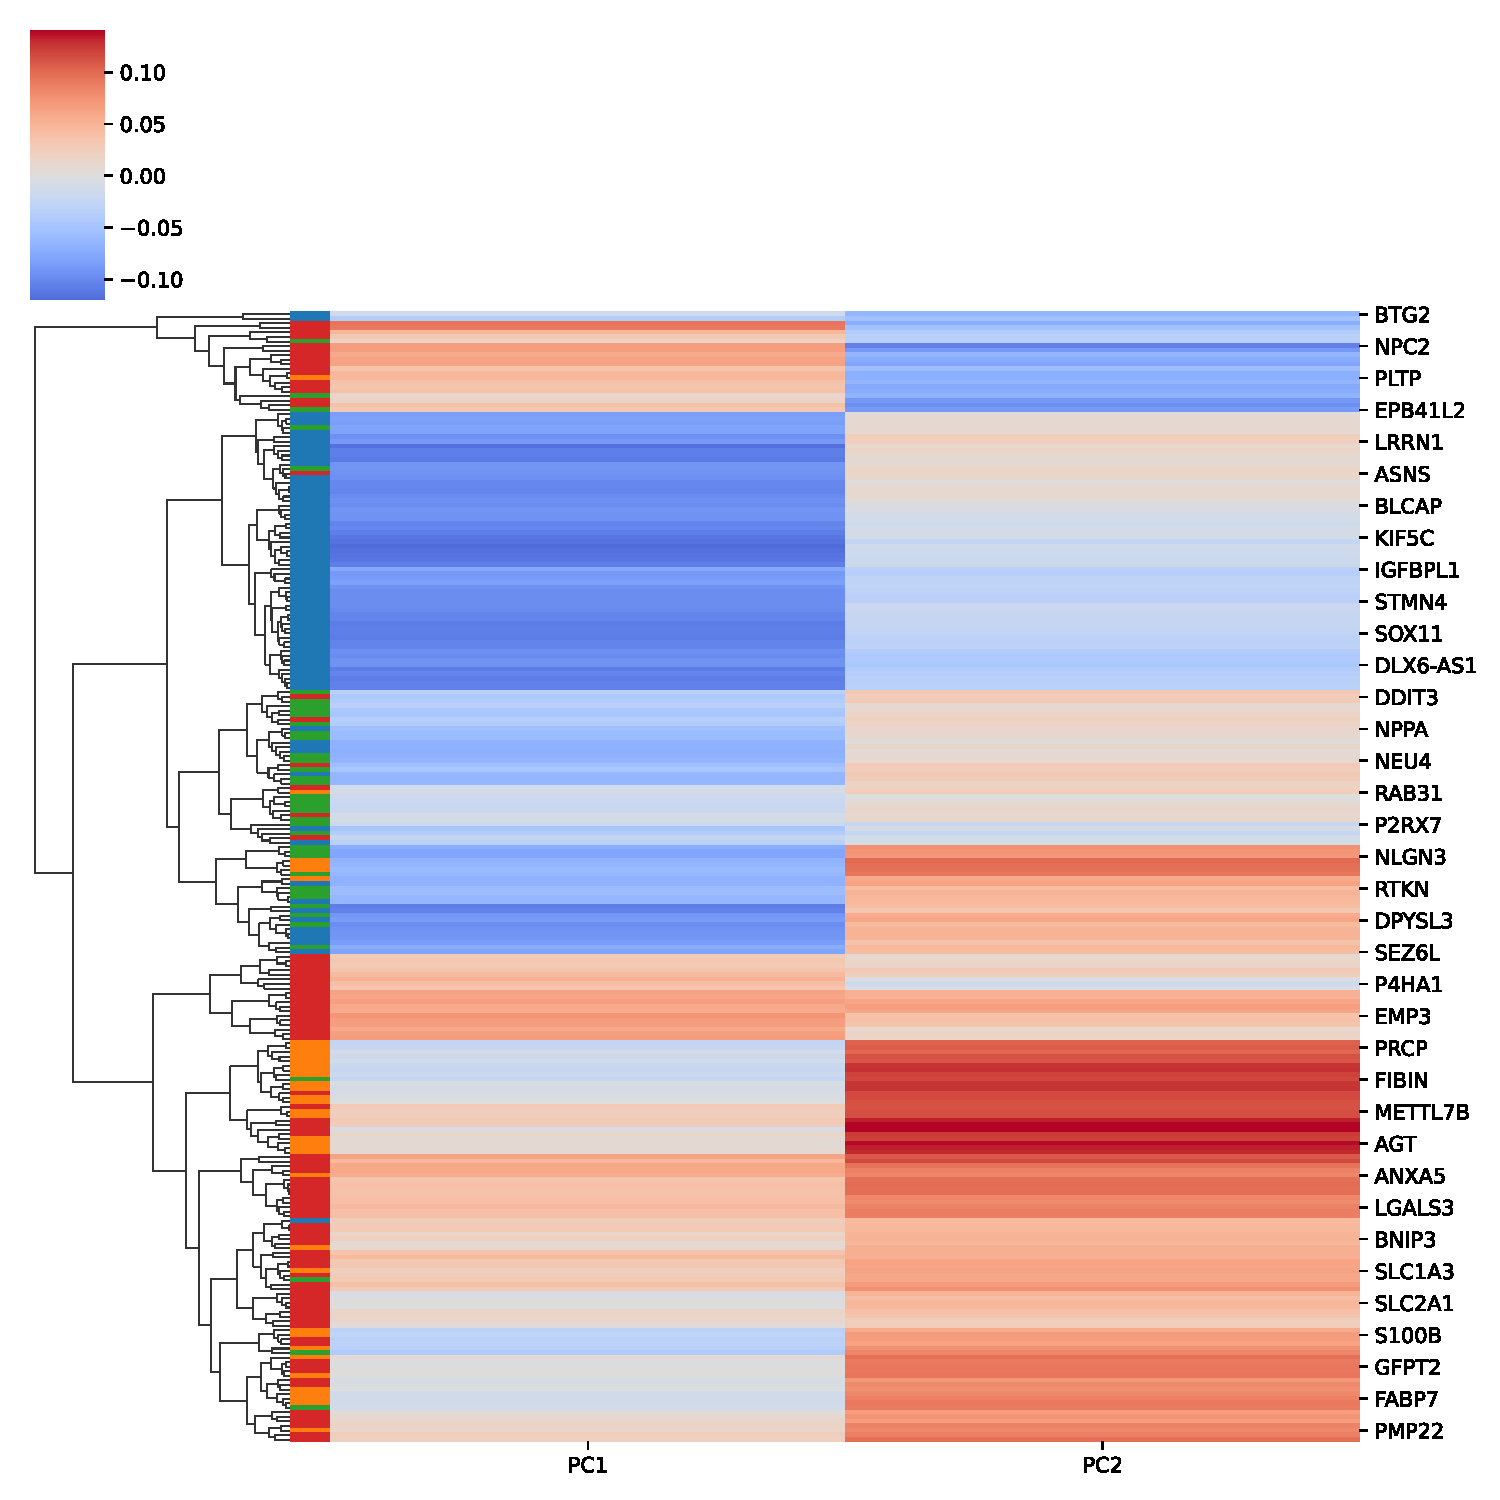
\includegraphics[width=\textwidth]{GSM3828673_loadings_plot}
                    \caption{GSE131928 - GSM3828673 (10X)}
                \end{subfigure}
                \caption{Loadings of PCA on signature expression}
            \end{figure}
        \end{adjustwidth}
    \end{frame}

    \begin{frame}{Signature PCA}
        \begin{adjustwidth}{-5cm}{-5cm}
            \centering
            \begin{figure}\ContinuedFloat
                \centering
                \begin{subfigure}[b]{0.38\textwidth}
                    \centering
                    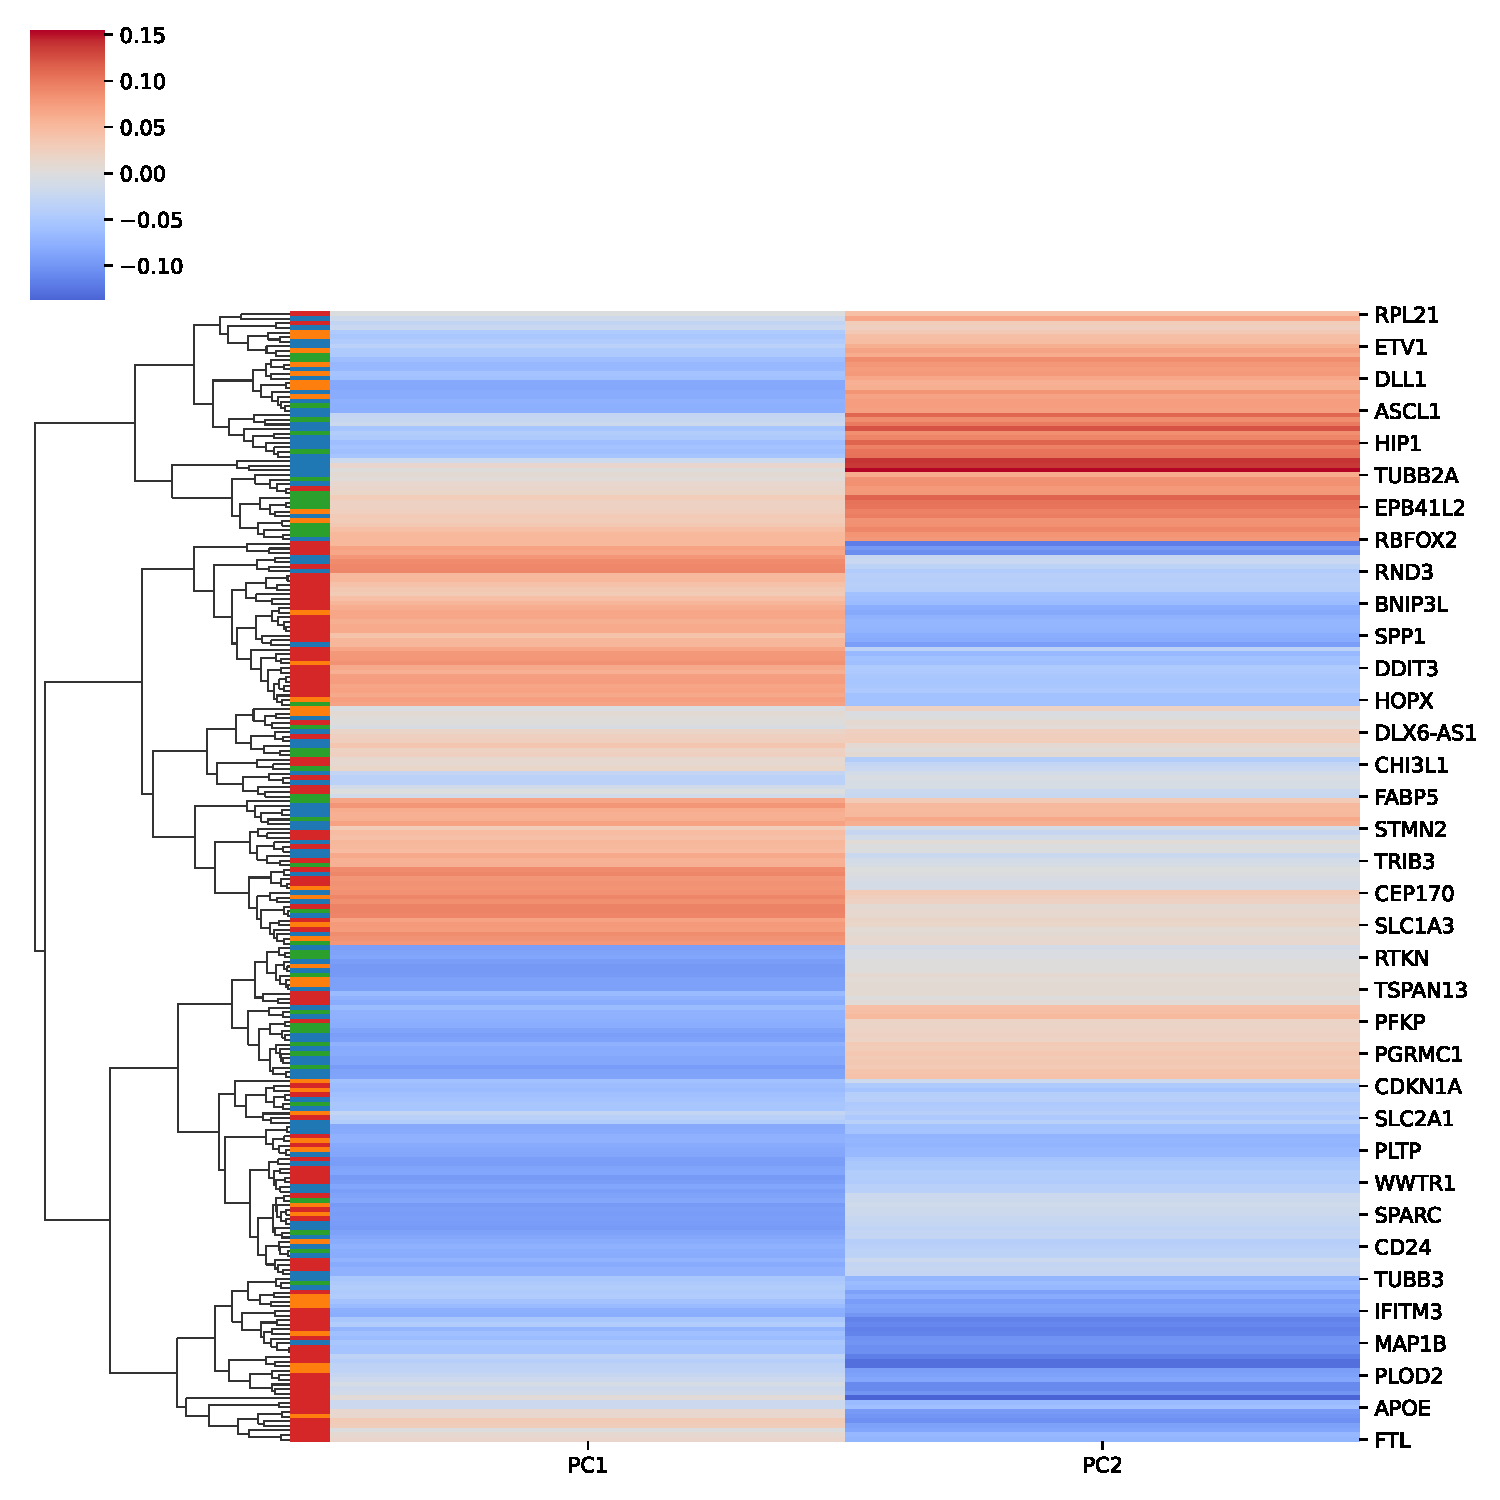
\includegraphics[width=\textwidth]{OSM_celllines_loadings_plot}
                    \caption{GSE168004 - OSM (treated)}
                \end{subfigure}
                \begin{subfigure}[b]{0.38\textwidth}
                    \centering
                    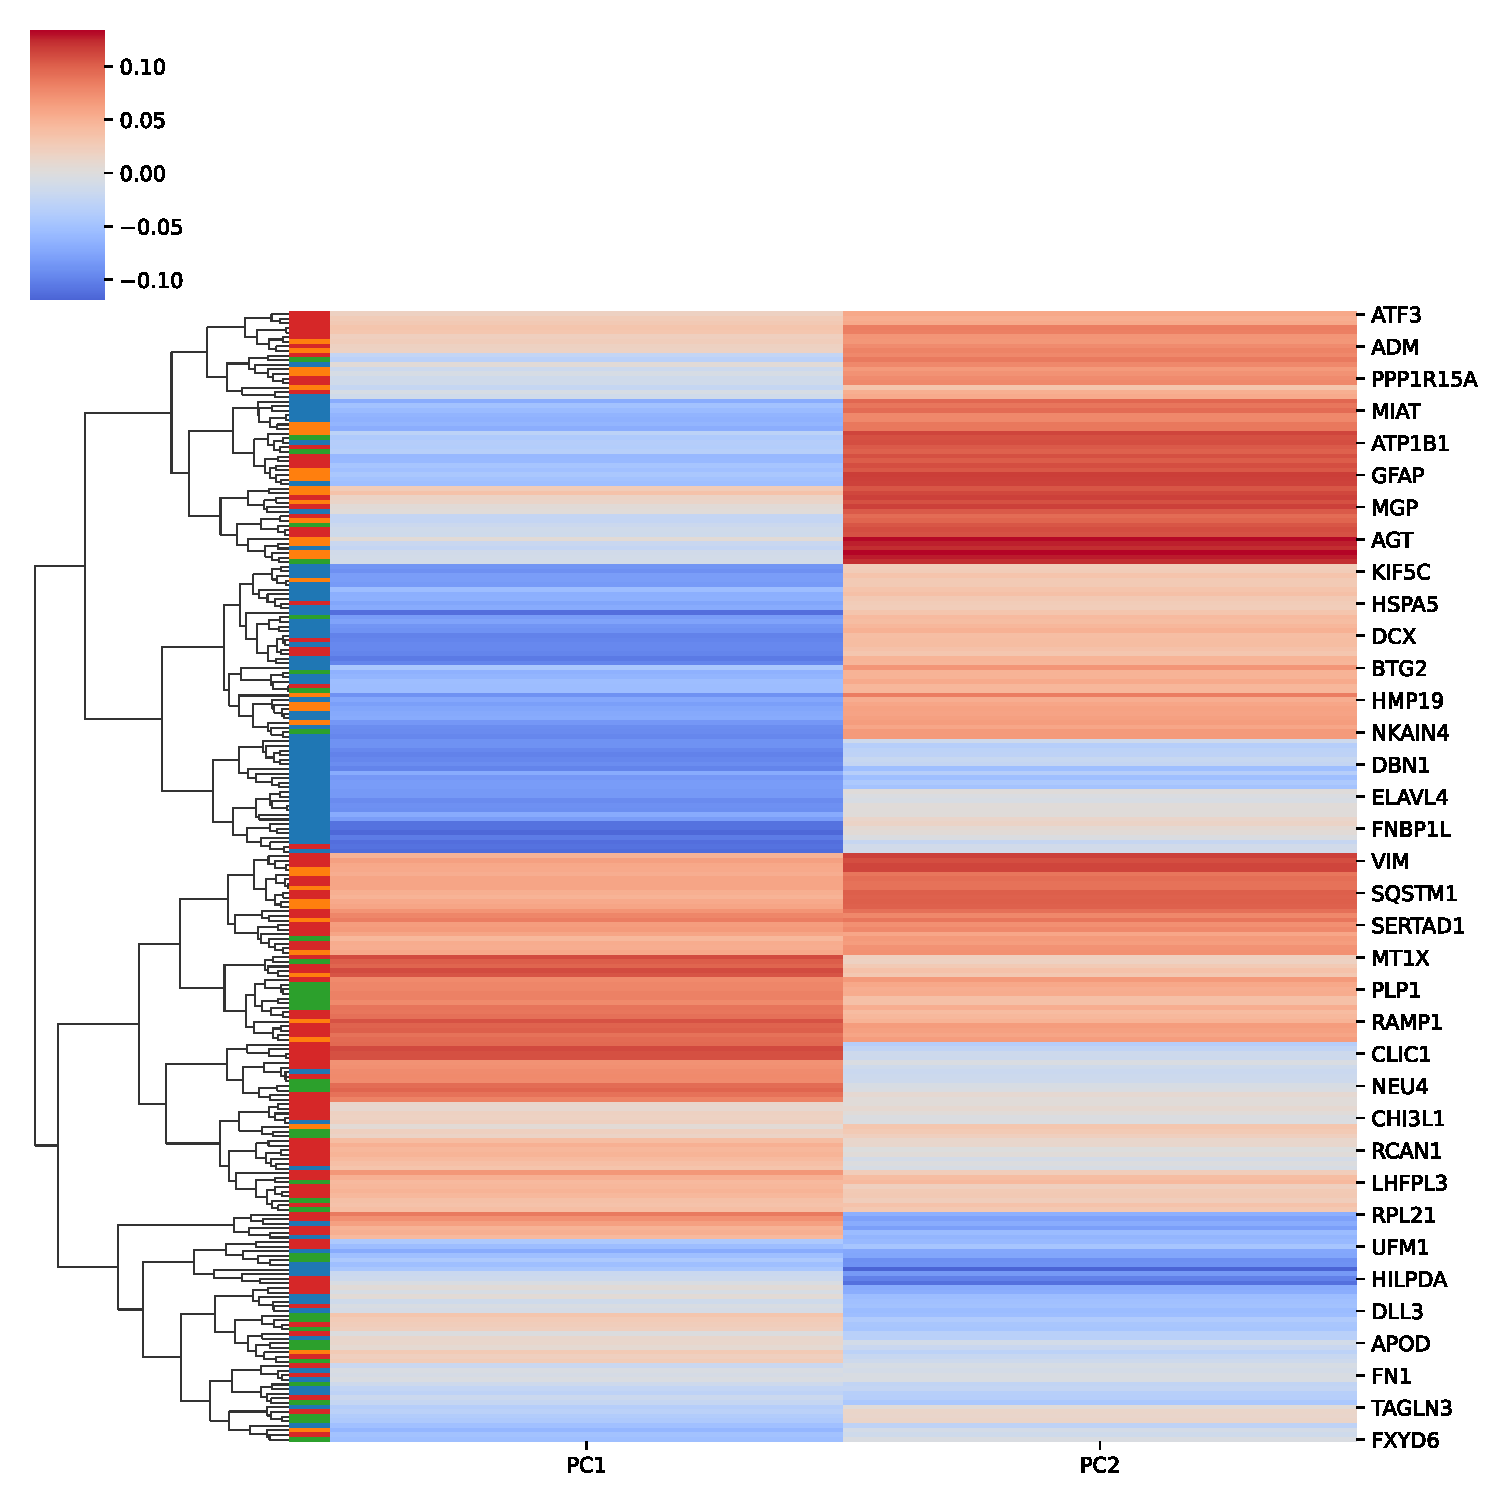
\includegraphics[width=\textwidth]{mgg23_loadings_plot}
                    \caption{GSE168004 - mgg23 (Control)}
                \end{subfigure}
                \begin{subfigure}[b]{0.38\textwidth}
                    \centering
                    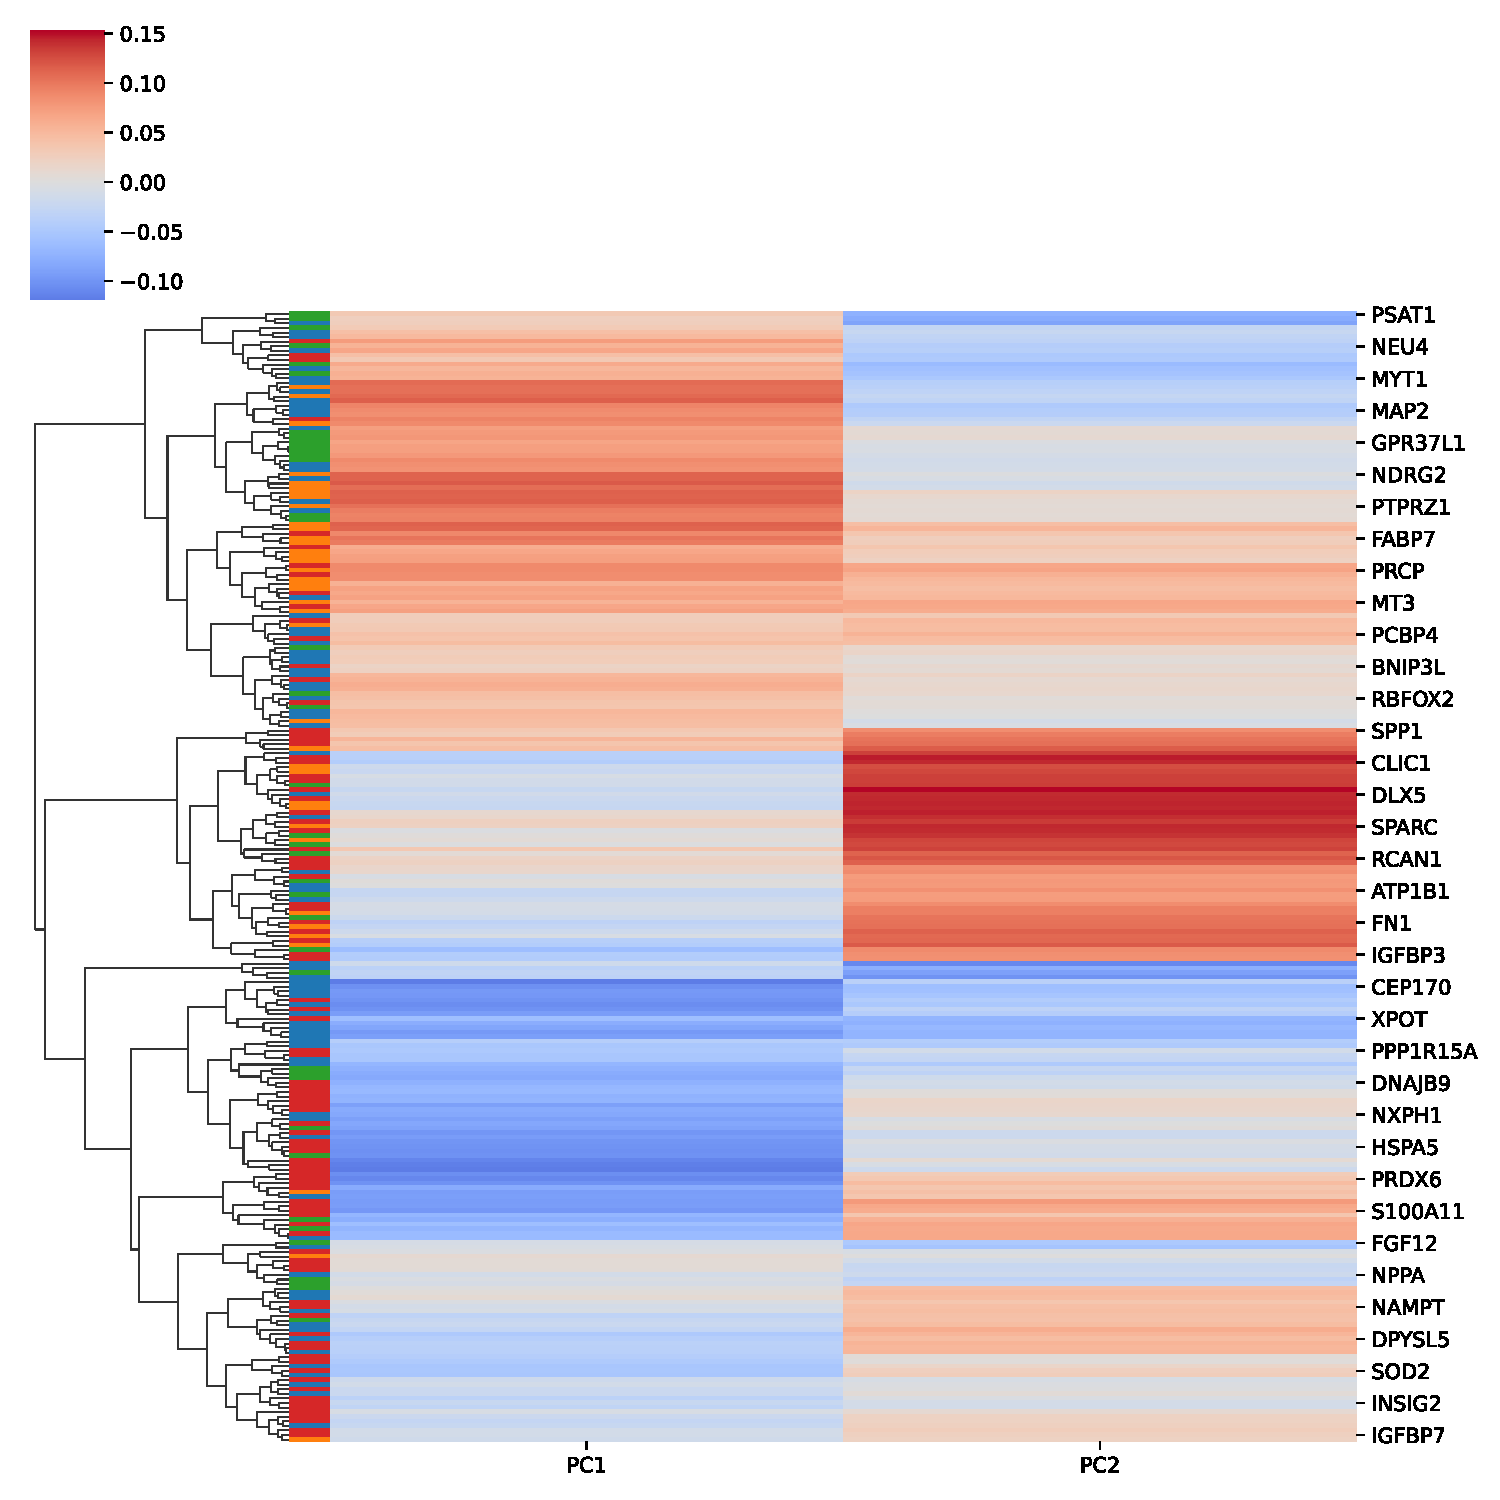
\includegraphics[width=\textwidth]{mgg75_loadings_plot}
                    \caption{GSE168004 - mgg75 (Control)}
                \end{subfigure}
                \caption{Loadings of PCA on signature expression}
            \end{figure}
        \end{adjustwidth}
    \end{frame}

    \begin{frame}{PCA correlation with AUCell scores}
        \begin{adjustwidth}{-5cm}{-5cm}
            \centering
            \begin{figure}
                \centering
                \begin{subfigure}[b]{0.38\textwidth}
                    \centering
                    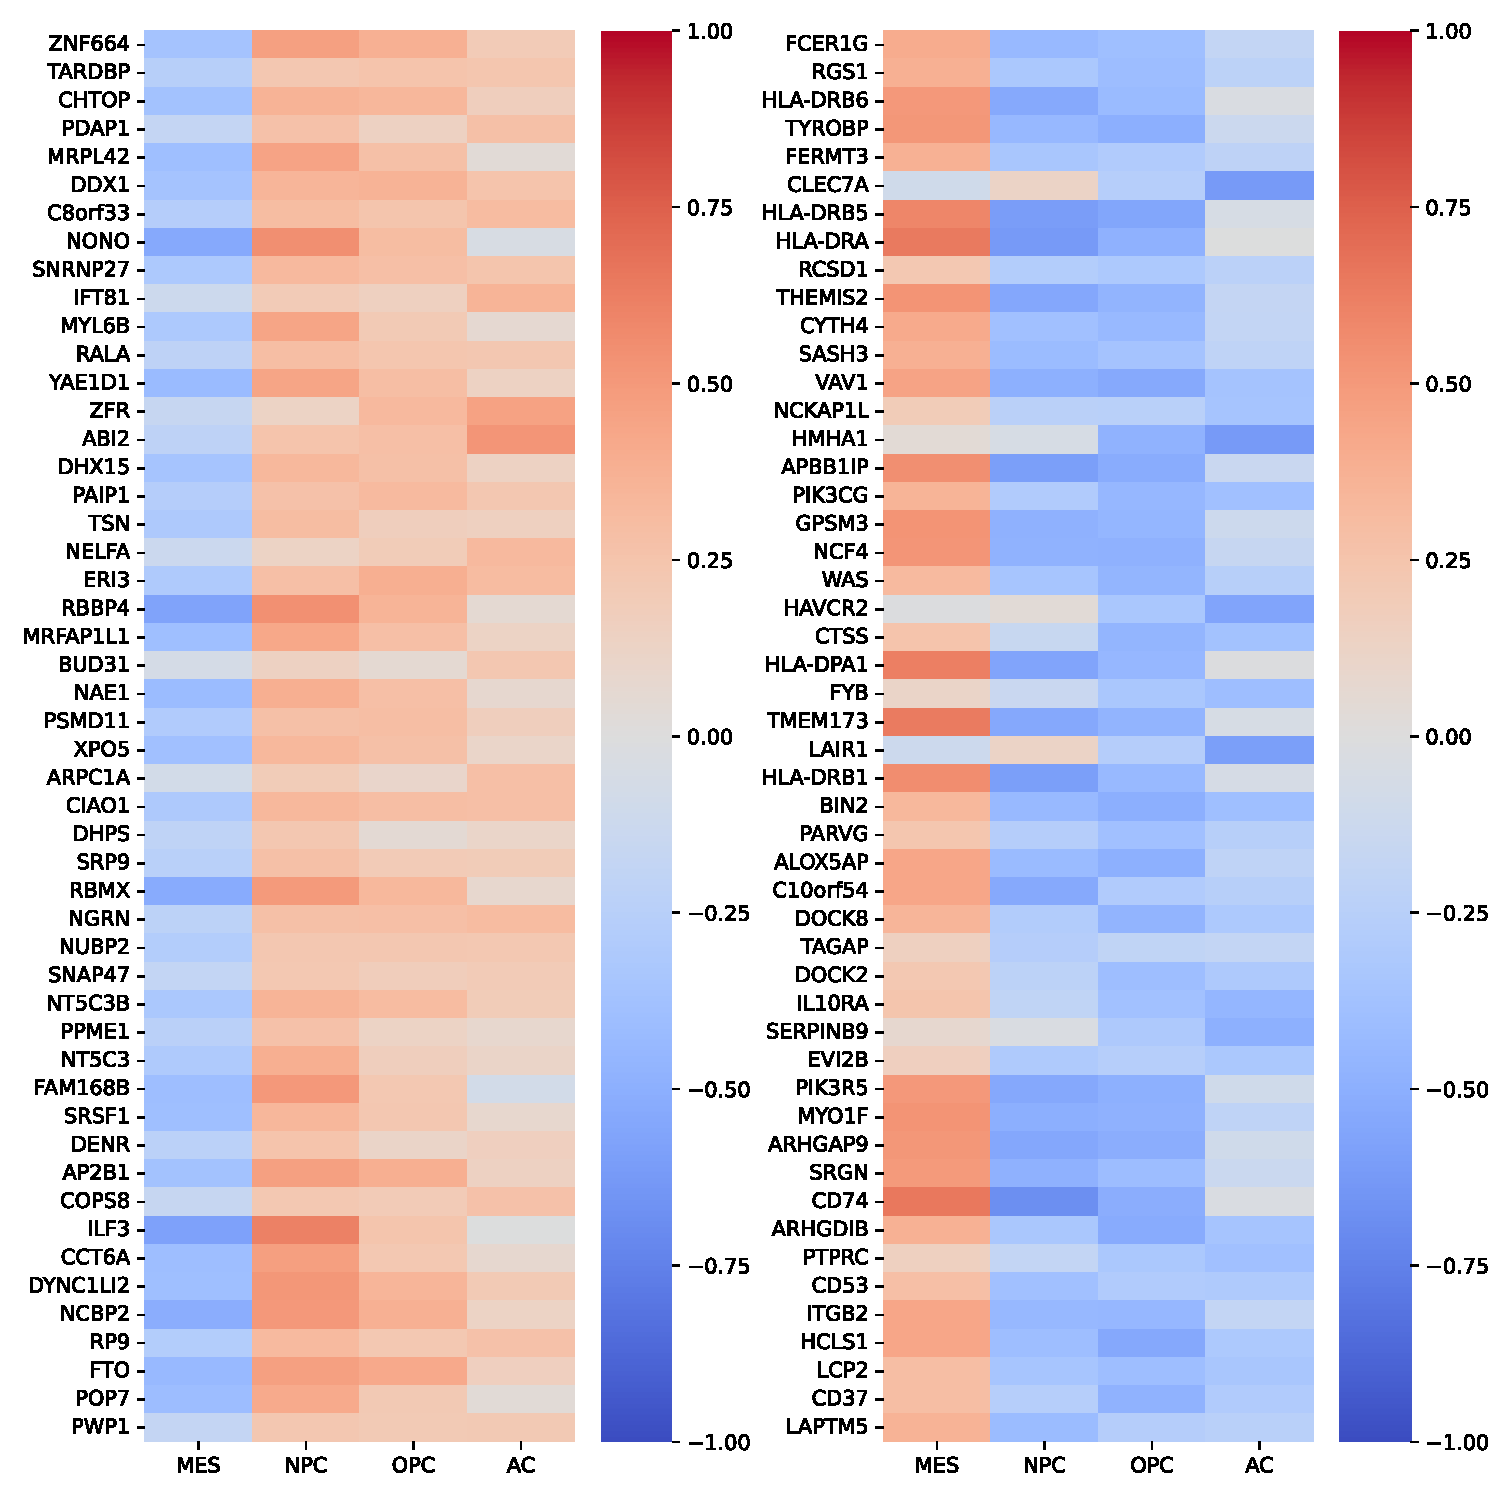
\includegraphics[width=\textwidth]{GSM3828672_load-corr}
                    \caption{GSE131928 - GSM3828672 (Smartseq2)}
                \end{subfigure}
                \begin{subfigure}[b]{0.38\textwidth}
                    \centering
                    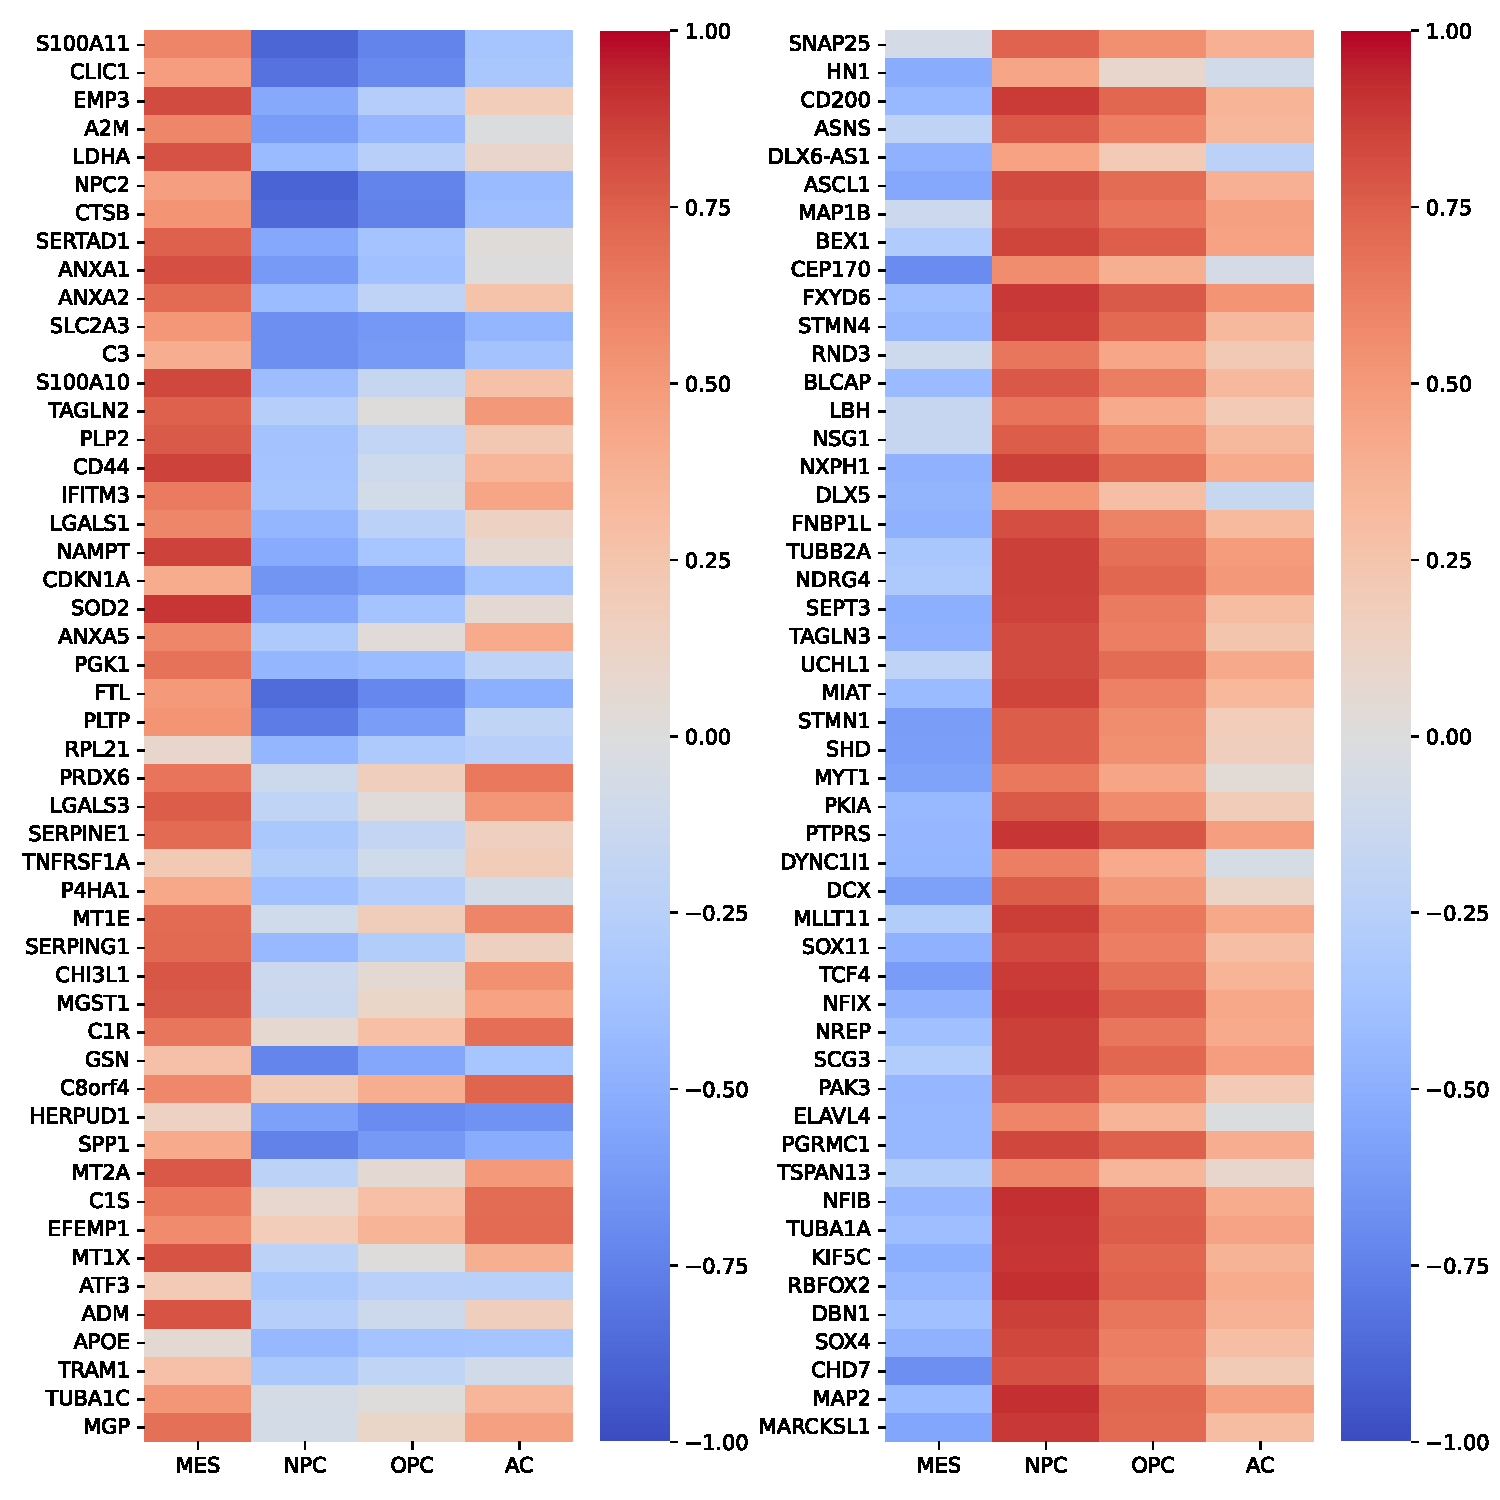
\includegraphics[width=\textwidth]{GSM3828673_load-corr}
                    \caption{GSE131928 - GSM3828673 (10X)}
                \end{subfigure}
                \caption{Correlation of top loading PCA with AUCell scores}
            \end{figure}
        \end{adjustwidth}
    \end{frame}

    \begin{frame}{PCA correlation with AUCell scores}
        \begin{adjustwidth}{-5cm}{-5cm}
            \centering
            \begin{figure}\ContinuedFloat
                \centering
                \begin{subfigure}[b]{0.38\textwidth}
                    \centering
                    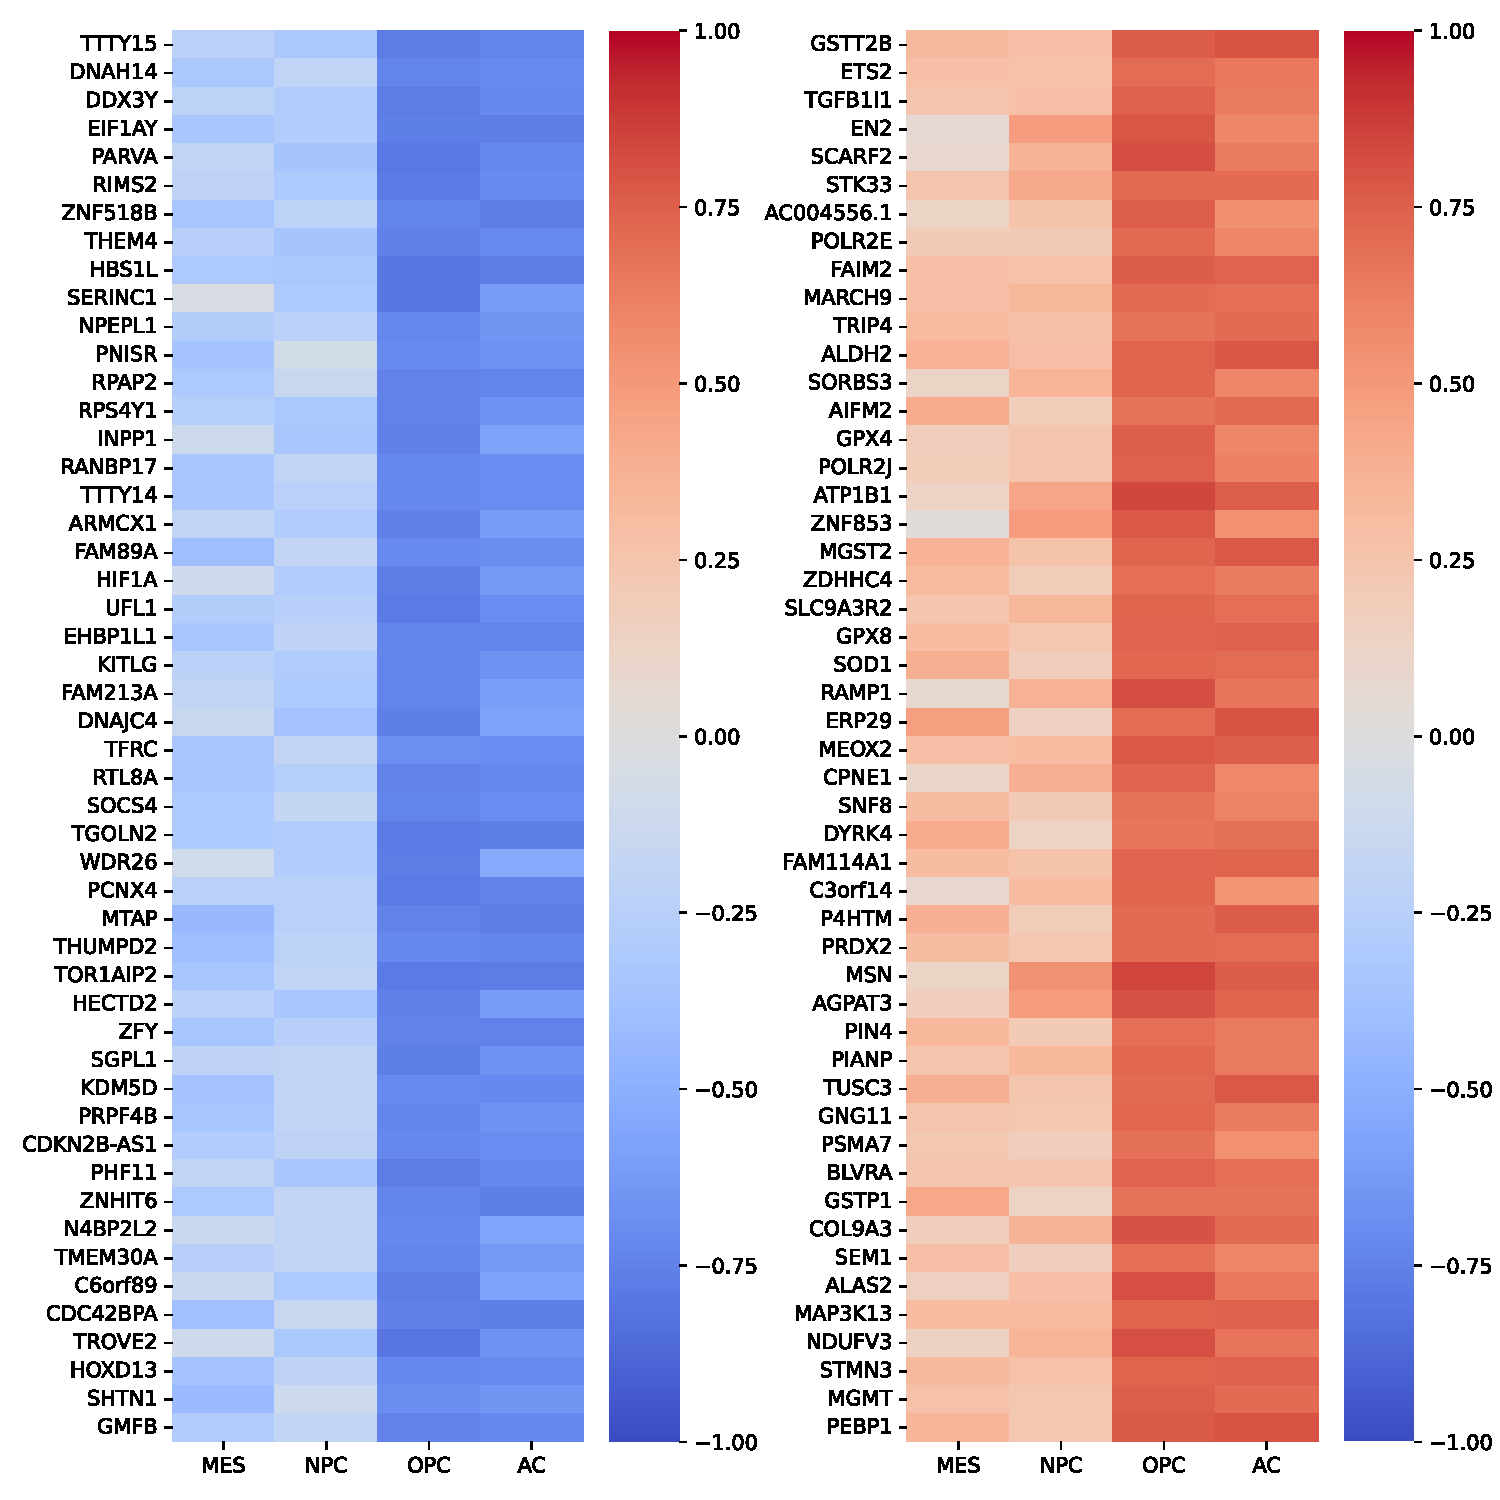
\includegraphics[width=\textwidth]{OSM_celllines_load-corr}
                    \caption{GSE168004 - OSM (treated)}
                \end{subfigure}
                \begin{subfigure}[b]{0.38\textwidth}
                    \centering
                    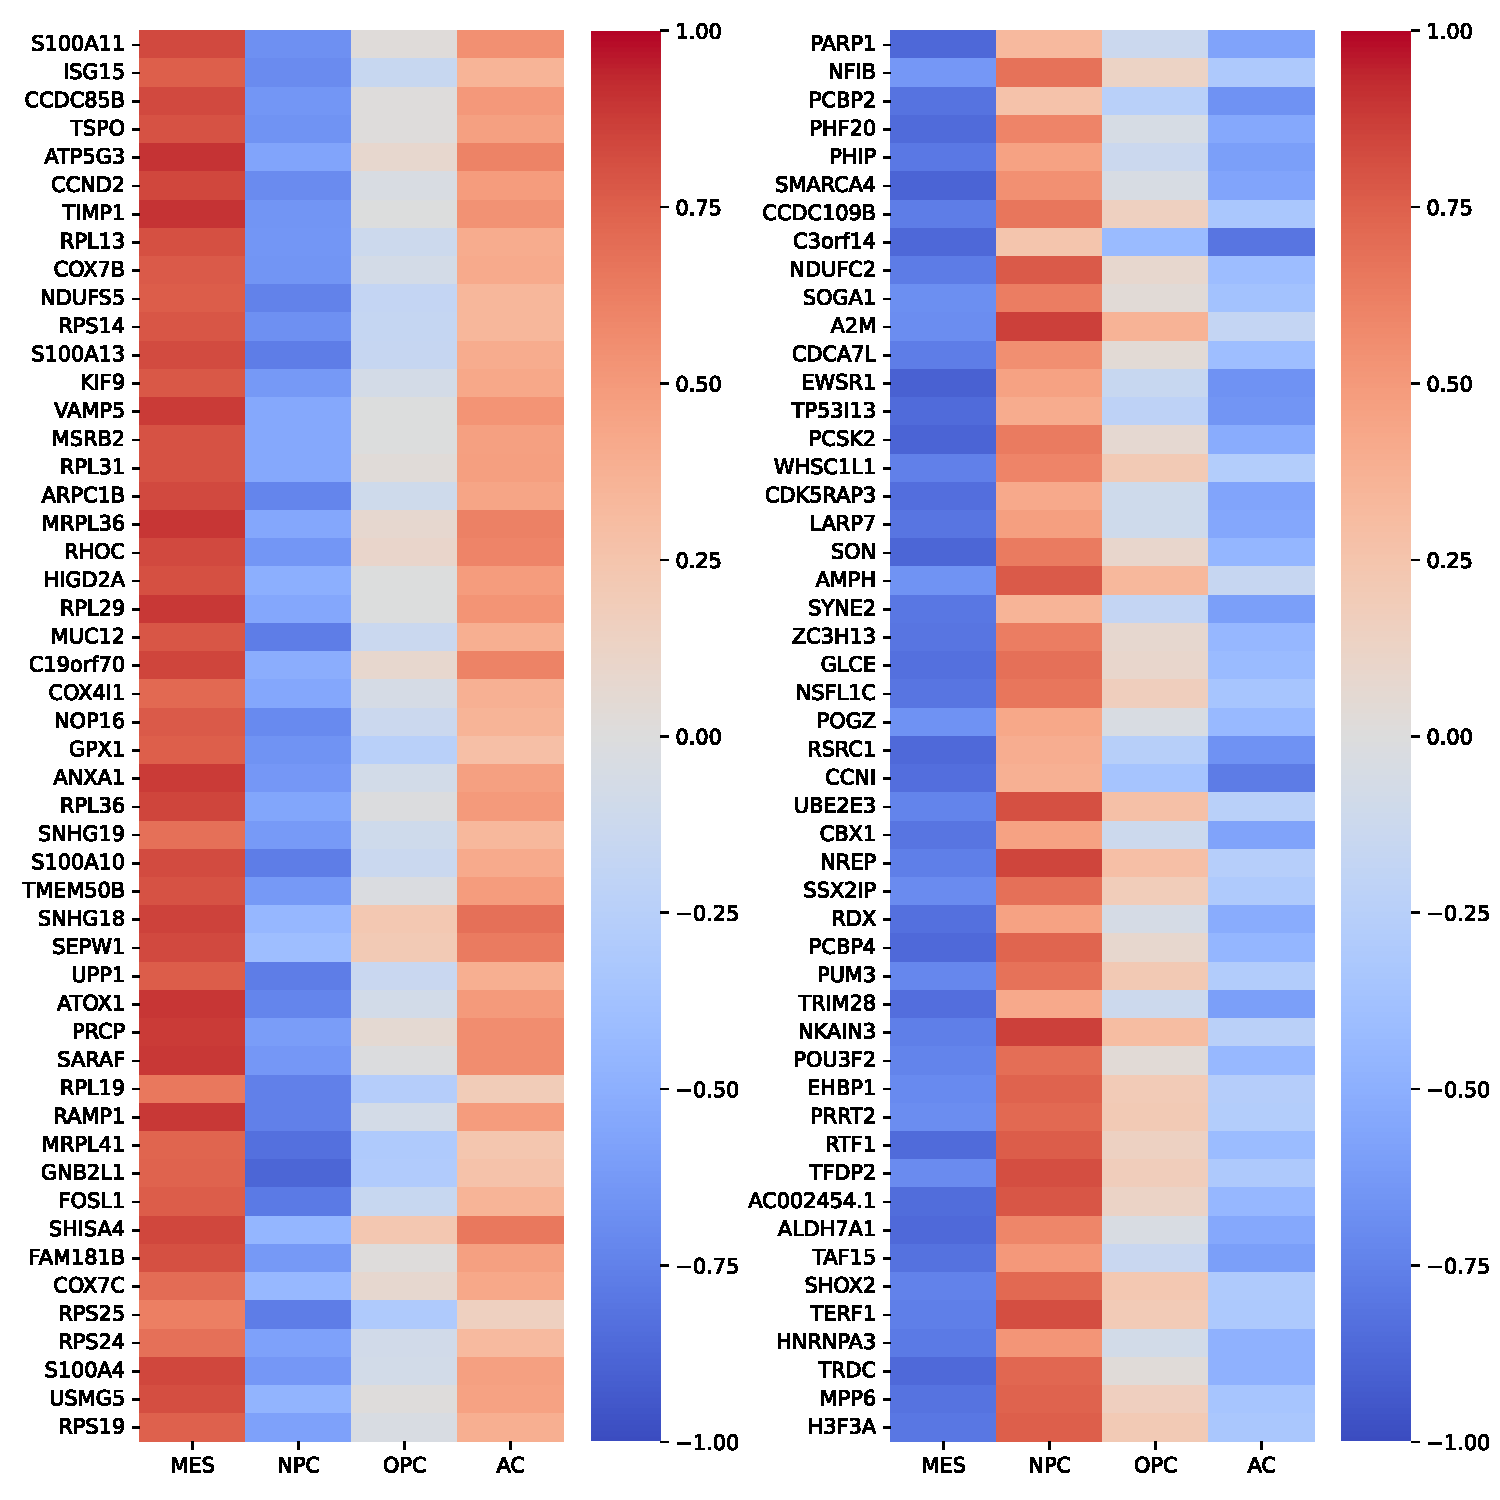
\includegraphics[width=\textwidth]{mgg23_load-corr}
                    \caption{GSE168004 - mgg23 (Control)}
                \end{subfigure}
                \begin{subfigure}[b]{0.38\textwidth}
                    \centering
                    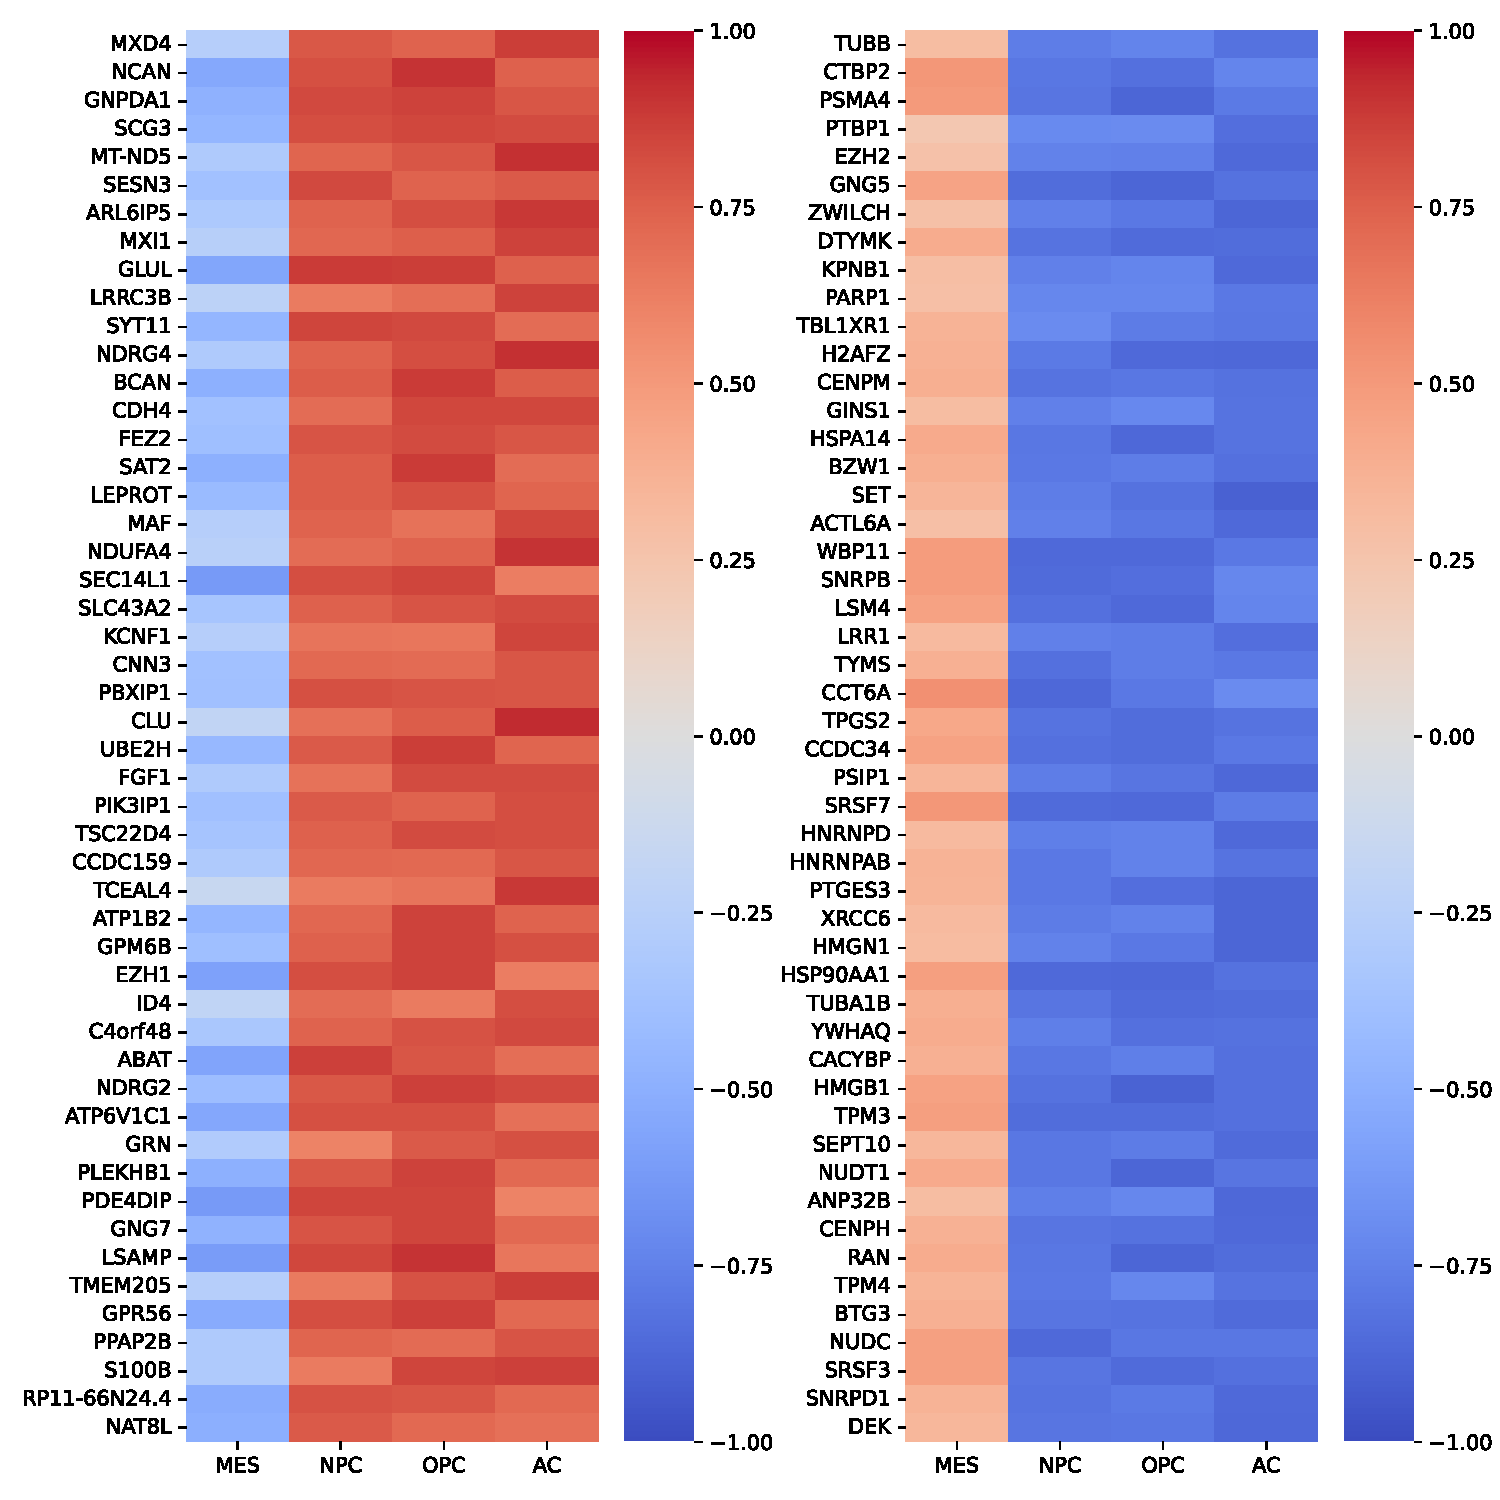
\includegraphics[width=\textwidth]{mgg75_load-corr}
                    \caption{GSE168004 - mgg75 (Control)}
                \end{subfigure}
                \caption{Correlation of top loading PCA with AUCell score}
            \end{figure}
        \end{adjustwidth}
    \end{frame}

\end{document}

